% Options for packages loaded elsewhere
% Options for packages loaded elsewhere
\PassOptionsToPackage{unicode}{hyperref}
\PassOptionsToPackage{hyphens}{url}
\PassOptionsToPackage{dvipsnames,svgnames,x11names}{xcolor}
%
\documentclass[review,
  12pt,
]{elsarticle}
\usepackage{xcolor}
\usepackage[left=25mm,right=25mm,top=25mm,bottom=25mm]{geometry}
\usepackage{amsmath,amssymb}
\setcounter{secnumdepth}{-\maxdimen} % remove section numbering
\usepackage{iftex}
\ifPDFTeX
  \usepackage[T1]{fontenc}
  \usepackage[utf8]{inputenc}
  \usepackage{textcomp} % provide euro and other symbols
\else % if luatex or xetex
  \usepackage{unicode-math} % this also loads fontspec
  \defaultfontfeatures{Scale=MatchLowercase}
  \defaultfontfeatures[\rmfamily]{Ligatures=TeX,Scale=1}
\fi
\usepackage{lmodern}
\ifPDFTeX\else
  % xetex/luatex font selection
\fi
% Use upquote if available, for straight quotes in verbatim environments
\IfFileExists{upquote.sty}{\usepackage{upquote}}{}
\IfFileExists{microtype.sty}{% use microtype if available
  \usepackage[]{microtype}
  \UseMicrotypeSet[protrusion]{basicmath} % disable protrusion for tt fonts
}{}
\makeatletter
\@ifundefined{KOMAClassName}{% if non-KOMA class
  \IfFileExists{parskip.sty}{%
    \usepackage{parskip}
  }{% else
    \setlength{\parindent}{0pt}
    \setlength{\parskip}{6pt plus 2pt minus 1pt}}
}{% if KOMA class
  \KOMAoptions{parskip=half}}
\makeatother
% Make \paragraph and \subparagraph free-standing
\makeatletter
\ifx\paragraph\undefined\else
  \let\oldparagraph\paragraph
  \renewcommand{\paragraph}{
    \@ifstar
      \xxxParagraphStar
      \xxxParagraphNoStar
  }
  \newcommand{\xxxParagraphStar}[1]{\oldparagraph*{#1}\mbox{}}
  \newcommand{\xxxParagraphNoStar}[1]{\oldparagraph{#1}\mbox{}}
\fi
\ifx\subparagraph\undefined\else
  \let\oldsubparagraph\subparagraph
  \renewcommand{\subparagraph}{
    \@ifstar
      \xxxSubParagraphStar
      \xxxSubParagraphNoStar
  }
  \newcommand{\xxxSubParagraphStar}[1]{\oldsubparagraph*{#1}\mbox{}}
  \newcommand{\xxxSubParagraphNoStar}[1]{\oldsubparagraph{#1}\mbox{}}
\fi
\makeatother


\usepackage{longtable,booktabs,array}
\usepackage{calc} % for calculating minipage widths
% Correct order of tables after \paragraph or \subparagraph
\usepackage{etoolbox}
\makeatletter
\patchcmd\longtable{\par}{\if@noskipsec\mbox{}\fi\par}{}{}
\makeatother
% Allow footnotes in longtable head/foot
\IfFileExists{footnotehyper.sty}{\usepackage{footnotehyper}}{\usepackage{footnote}}
\makesavenoteenv{longtable}
\usepackage{graphicx}
\makeatletter
\newsavebox\pandoc@box
\newcommand*\pandocbounded[1]{% scales image to fit in text height/width
  \sbox\pandoc@box{#1}%
  \Gscale@div\@tempa{\textheight}{\dimexpr\ht\pandoc@box+\dp\pandoc@box\relax}%
  \Gscale@div\@tempb{\linewidth}{\wd\pandoc@box}%
  \ifdim\@tempb\p@<\@tempa\p@\let\@tempa\@tempb\fi% select the smaller of both
  \ifdim\@tempa\p@<\p@\scalebox{\@tempa}{\usebox\pandoc@box}%
  \else\usebox{\pandoc@box}%
  \fi%
}
% Set default figure placement to htbp
\def\fps@figure{htbp}
\makeatother


% definitions for citeproc citations
\NewDocumentCommand\citeproctext{}{}
\NewDocumentCommand\citeproc{mm}{%
  \begingroup\def\citeproctext{#2}\cite{#1}\endgroup}
\makeatletter
 % allow citations to break across lines
 \let\@cite@ofmt\@firstofone
 % avoid brackets around text for \cite:
 \def\@biblabel#1{}
 \def\@cite#1#2{{#1\if@tempswa , #2\fi}}
\makeatother
\newlength{\cslhangindent}
\setlength{\cslhangindent}{1.5em}
\newlength{\csllabelwidth}
\setlength{\csllabelwidth}{3em}
\newenvironment{CSLReferences}[2] % #1 hanging-indent, #2 entry-spacing
 {\begin{list}{}{%
  \setlength{\itemindent}{0pt}
  \setlength{\leftmargin}{0pt}
  \setlength{\parsep}{0pt}
  % turn on hanging indent if param 1 is 1
  \ifodd #1
   \setlength{\leftmargin}{\cslhangindent}
   \setlength{\itemindent}{-1\cslhangindent}
  \fi
  % set entry spacing
  \setlength{\itemsep}{#2\baselineskip}}}
 {\end{list}}
\usepackage{calc}
\newcommand{\CSLBlock}[1]{\hfill\break\parbox[t]{\linewidth}{\strut\ignorespaces#1\strut}}
\newcommand{\CSLLeftMargin}[1]{\parbox[t]{\csllabelwidth}{\strut#1\strut}}
\newcommand{\CSLRightInline}[1]{\parbox[t]{\linewidth - \csllabelwidth}{\strut#1\strut}}
\newcommand{\CSLIndent}[1]{\hspace{\cslhangindent}#1}



\setlength{\emergencystretch}{3em} % prevent overfull lines

\providecommand{\tightlist}{%
  \setlength{\itemsep}{0pt}\setlength{\parskip}{0pt}}

\usepackage{indentfirst}
\setlength{\parindent}{15pt}
\setlength{\parskip}{10pt}
\usepackage[font=small]{caption}  % Options: small, footnotesize, scriptsize, etc.
%\usepackage[noblocks]{authblk}
%\renewcommand*{\Authsep}{, }
%\renewcommand*{\Authand}{, }
%\renewcommand*{\Authands}{, }
%\renewcommand\Affilfont{\small}
% Define a keywords command for inline keywords
%\newcommand{\printkeywords}[1]{\noindent\textbf{Keywords:} #1\par}
\makeatletter
\@ifpackageloaded{caption}{}{\usepackage{caption}}
\AtBeginDocument{%
\ifdefined\contentsname
  \renewcommand*\contentsname{Table of contents}
\else
  \newcommand\contentsname{Table of contents}
\fi
\ifdefined\listfigurename
  \renewcommand*\listfigurename{List of Figures}
\else
  \newcommand\listfigurename{List of Figures}
\fi
\ifdefined\listtablename
  \renewcommand*\listtablename{List of Tables}
\else
  \newcommand\listtablename{List of Tables}
\fi
\ifdefined\figurename
  \renewcommand*\figurename{Figure}
\else
  \newcommand\figurename{Figure}
\fi
\ifdefined\tablename
  \renewcommand*\tablename{Table}
\else
  \newcommand\tablename{Table}
\fi
}
\@ifpackageloaded{float}{}{\usepackage{float}}
\floatstyle{ruled}
\@ifundefined{c@chapter}{\newfloat{codelisting}{h}{lop}}{\newfloat{codelisting}{h}{lop}[chapter]}
\floatname{codelisting}{Listing}
\newcommand*\listoflistings{\listof{codelisting}{List of Listings}}
\makeatother
\makeatletter
\makeatother
\makeatletter
\@ifpackageloaded{caption}{}{\usepackage{caption}}
\@ifpackageloaded{subcaption}{}{\usepackage{subcaption}}
\makeatother
\usepackage{bookmark}
\IfFileExists{xurl.sty}{\usepackage{xurl}}{} % add URL line breaks if available
\urlstyle{same}
\hypersetup{
  pdftitle={Neural responses to binocular in-phase and anti-phase stimuli},
  pdfauthor={Bruno Richard; Daniel H. Baker},
  colorlinks=true,
  linkcolor={blue},
  filecolor={Maroon},
  citecolor={Blue},
  urlcolor={Blue},
  pdfcreator={LaTeX via pandoc}}

\begin{document}

\begin{frontmatter}

\title{Neural responses to binocular in-phase and anti-phase stimuli}

\author[inst1]{Bruno Richard\corref{cor1}}
\cortext[cor1]{Corresponding author}
\ead{br379@newark.rutgers.edu}

\author[inst2]{Daniel H. Baker}

\address[inst1]{Department of Math and Computer Sciences, Rutgers University, Newark, New Jersey, USA}
\address[inst2]{Department of Psychology, University of York, York, UK}

\begin{abstract}
Binocular vision fuses similar inputs from the two eyes into a single
percept, whereas incompatible inputs can produce rivalry, lustre, or
diplopia. We measured neural responses to binocular stimuli with
different phase relationships to test predictions from contemporary
binocular combination models. Steady-State Visually Evoked Potentials
(SSVEPs) were recorded from 15 observers in response to monocular and
binocular stimulation at 3 Hz, using either On/Off or counterphase
flicker with varied spatial and temporal phase relationships. On/Off and
counterphase flicker elicited responses at the expected fundamental
frequency (3 Hz and 6 Hz, respectively) and their harmonics.
Manipulating phase relationships modulated these response patterns,
including a reduction in the fundamental amplitude for On/Off flicker.
The data were modeled with a series of binocular combination algorithms,
ranging in complexity from a simple linear sum to a two-stage binocular
gain-control model with parallel monocular and binocular phase-selective
channels. The model required parallel monocular channels to account for
our data, whereas phase selectivity was not essential. Overall, the
two-stage contrast gain-control model remains a powerful and flexible
framework for describing binocular combinations across various
experimental conditions and modalities.
\end{abstract}

\begin{keyword}
Binocular Combination \sep SSVEP \sep Contrast Gain Control \sep Phase Selectivity \sep Monocular Channels
\end{keyword}

\end{frontmatter}


%\title{Neural responses to binocular in-phase and anti-phase stimuli}

%  \author[1]{Bruno Richard}
%  \author[2]{Daniel H. Baker}

%      \affil[1]{Department of Math and Computer Sciences, Rutgers
%University, Newark, New Jersey, USA}
%      \affil[2]{Department of Psychology, University of York, York, UK}
  

\section{Introduction}\label{introduction}

The human visual system integrates input from both eyes to form a
unified binocular representation of the world. Combining monocular
inputs enhances sensitivity to the presented stimuli, particularly when
the contrast is low or near detection threshold (Baker et al., 2018;
Campbell and Green, 1965; Meese et al., 2006). Contrast sensitivity can
improve by a factor of \(\sqrt{2}\) or more when stimuli are presented
binocularly versus monocularly (Baker et al., 2018; Blake and Wilson,
2011; Campbell and Green, 1965; Richard et al., 2018). Notably, the
visual system also attempts to combine inputs even when the stimuli
presented to each eye are markedly different (i.e., incompatible). In
such cases, observers may perceive binocular rivalry (Blake, 1989;
Wilson, 2003), diplopia, or visual lustre (Wendt and Faul, 2022).
Despite differences in perceptual outcomes, computationally, the
underlying processes of binocular combination for compatible and
incompatible inputs appear similar (Baker et al., 2007a; Legge, 1984a).
Psychophysical responses to compatible and incompatible stimuli can be
effectively explained by a single psychophysical model that involves
nonlinear transduction, followed by summation across monocular and
binocular phase-selective channels (Baker et al., 2007a; Baker and
Meese, 2007). Here, we explore if the integrative processes defined over
multiple behavioural tasks are also reflected at the neural level.

It has long been known that stimuli presented binocularly are summed
across the eyes. In contrast detection tasks, where stimulus contrast is
low, binocular presentation increases sensitivity by approximately
\(\sqrt{2}\) (Campbell and Green, 1965). This implies that observers
require roughly 1.4 times more contrast to detect a monocular stimulus
than a binocular one. The binocular improvement in sensitivity is
consistent with a non-linearity operating before the signals from the
two eyes (\(C_L\) and \(C_R\)) are combined (Legge, 1984a):
\begin{equation}\phantomsection\label{eq-IntroMath1}{
R_B = C_L^m + C_R^m.
}\end{equation} Here, the exponent \(m\) determines the degree of
summation. When \(m = 1\), summation is linear, yielding a doubling of
sensitivity. When \(m = 2\), summation is reduced to \(\sqrt{2}\).
Several studies have reported summation ratios over \(\sqrt{2}\) with
some approaching 1.8 (Meese et al., 2006; Simmons, 2005; Simmons and
Kingdom, 1998). A recent meta-analysis of 65 studies (N = 716) found an
average binocular summation ratio of 1.5 (Baker et al., 2018). This work
highlighted the challenges in accurately describing the binocular
summation process (e.g., \(m\)) as individual variability and
methodological differences can greatly impact binocular summation.

The contrast of stimuli is crucial in measuring binocular summation.
Binocular summation can be very large when stimulus contrast is low;
however, the binocular advantage is seldom observed in tasks that
involve higher contrasts. In contrast discrimination tasks, where
observers judge the contrast difference between otherwise identical
stimuli, binocular presentation no longer confers a benefit in
sensitivity: discrimination thresholds are identical whether stimuli are
shown to one eye or both (Legge, 1984a; Maehara and Goryo, 2005; Meese
et al., 2006). However, this does not indicate that binocular summation
does not occur at higher contrasts; the monocular signals are still
summed (Meese et al., 2006; Meese and Baker, 2011). Instead, the
advantage of summation is counteracted by normalization mechanisms that
maintain consistency across viewing conditions (referred to as
`ocularity invariance'). In gain control models of early vision,
normalization can stem from interocular and self-suppressive signals
(Meese et al., 2006):
\begin{equation}\phantomsection\label{eq-intoMath2}{
R_B = \frac{C_L^m}{S+C_L+C_R} + \frac{C_R^m}{S+C_R+C_L}.
}\end{equation} When both eyes are stimulated, the suppressive terms on
the denominators offset the enhanced excitatory signals, nullifying the
binocular advantage.

A similar pattern of results is observed in neural measurements of
binocular summation. In functional Magnetic Resonance Imaging (fMRI)
recordings, neural responses are significantly larger for binocular than
monocular responses when stimulus contrast is low (Moradi and Heeger,
2009). At higher contrasts, observers no longer show the binocular
advantage. As with behavioural results, these findings are
well-explained computationally by interocular suppression and binocular
contrast normalization. The equivalency in binocular summation between
psychophysics and neuroimaging findings means that both data types can
constrain binocular summation models. We, for example, have previously
demonstrated that a popular model of binocular summation could be easily
adapted to capture Steady-State Visually Evoked Potentials (SSVEPs) to
monocular and binocular stimuli when one eye was occluded by a neutral
density filter (Richard et al., 2018). Placing a neutral density filter
in front of one eye darkens its input, reducing the amplitude and
altering the phase of SSVEPs to stimuli presented to the filtered eye.
Steady-State response amplitudes and phases to stimuli presented through
different neutral density filter strengths were well described by a
model that first used a biophysically plausible temporal filter on the
input stimuli, followed by self and interocular suppression, and
finally, binocular contrast normalization. This model also explained
psychophysically measured binocular summation in the same group of
observers. A comprehensive description of the processes involved in
binocular summation should be able to explain behavioural and
neuroimaging findings under various experimental conditions of binocular
summation.

Many studies have worked towards the development of a comprehensive
description of the process of binocular summation in human vision using
a variety of psychophysical and neuroimaging approaches (Baker et al.,
2008, 2007b; Ding et al., 2013; Ding and Sperling, 2006; Legge, 1984a;
Lygo et al., 2021; Maehara and Goryo, 2005; May and Zhaoping, 2016;
Richard et al., 2018). This is not an insignificant challenge; such a
description must account for multiple components of early vision,
including identifying relevant signals, defining how these signals might
interact, what non-linearities are present, and most importantly, how
these signals are summed and/or differenced. One model that has proven
very informative and capable of describing binocular summation under
various experimental conditions is the two-stage contrast gain control
model developed by Meese et al. (2006). In a two-stage process, the
model captured detection and discrimination thresholds for monocular and
binocular presentation, in addition to dichoptic masking (when the
stimuli presented to both eyes are not identical). First, the input is
rectified by an excitatory non-linearity (\(m \approx 1.3\)) and
normalized by self and interocular suppression (see
Equation~\ref{eq-intoMath2}). The binocular (e.g., combined) signal then
undergoes a second contrast normalization before the decision stage,
\begin{equation}\phantomsection\label{eq-IntroMathSecondStage}{
R = \frac{R_B^p}{Z + R_B^q},
}\end{equation} where the exponents \(p\) and \(q\) typically have quite
large values, and determine the shape of the contrast discrimination
(`dipper') functions.

Subsequent iterations of the two-stage contrast gain control model added
channels for opposite contrast polarities (Baker and Meese, 2007), and
monocular channels parallel to the binocular summing channel (Georgeson
et al., 2016). Polarity-specific channels were included to explain
masking effects when the stimuli presented to each eye had opposite
phase polarities (i.e., dichoptic presentation). Antiphase stimuli do
not cancel each other out (as would be expected if their luminances were
summed): the stimuli remain detectable and the two inputs can sum
(Bacon, 1976; Baker and Meese, 2007; Simmons, 2005), at least in a
probabilistic sense. Parallel monocular channels are consistent with
adaptation after-effects that suggest monocular signals may be preserved
and available for perception following binocular summation (Blake et
al., 1981; Moulden, 1980).

While the possibility of monocular channels had been considered (Legge,
1984a), many assumed that only the binocularly summed signal contributed
to perception. Georgeson et al. (2016) developed a specific experimental
condition to assess the involvement of monocular channels. They devised
a discrimination task where the target interval presented a contrast
increment to one eye (e.g., 10\% pedestal + 2\%) and a contrast
decrement to the other (e.g., 10\% pedestal - 2\%). If the only
available signal is a binocularly summed one, the task would be nearly
impossible to complete; the target interval would be perceptually
identical to the pedestal-only interval. However, observers were able to
complete the task. The two-stage contrast gain control model with
parallel monocular channels was the only model able to capture observer
thresholds from all experimental conditions, including the binocular
increment and decrement tasks. Evidence of an additional differencing
channel accompanying the summing channel commonly described in work on
binocular combination (Chen and Li, 1998; Li and Atick, 1994; May et
al., 2012; May and Zhaoping, 2016) has also accumulated. As the name
implies, this channel encodes the difference between stimuli presented
to the left and right eye; it is involved in early contributions to
disparity processing and stereovision. While computational models of
binocular vision do not explicitly include differencing channels,
encoding the difference between monocular signals is, indirectly,
included in the two-stage contrast gain control model defined by
Georgeson et al. (2016).

The current architecture of the two-stage contrast gain control model
has been rigorously evaluated on psychophysical data, providing a solid
foundation for our understanding of binocular combination (Baker and
Meese, 2007; Georgeson et al., 2016; Meese et al., 2006). While previous
studies have applied the two-stage contrast gain control model to
neuroimaging data (Lygo et al., 2021; Richard et al., 2018), they only
included experimental conditions where the phases of the sinusoidal
gratings presented to each eye were identical. To accurately assess the
current architecture of the two-stage contrast gain control model,
neuroimaging data for binocular presentation of stimuli in opposite
phase polarity are required. Here, we recorded SSVEPs to monocular and
binocular stimuli with different spatial and temporal phase
relationships to obtain the data needed to evaluate the two-stage
contrast gain control model. By progressively increasing the complexity
of the model, we demonstrate that many components of binocular
combination, such as monocular non-linearities, interocular
interactions, and parallel monocular channels, are required to explain
neural responses to our set of experimental conditions. The two-stage
contrast gain control model remains a powerful and flexible descriptor
of the architecture of binocular combination for data collected across
many experimental conditions and modalities.

\section{Methods}\label{methods}

\subsection{Participants}\label{participants}

Fifteen observers (including both authors: BR and DHB) with normal or
corrected to normal visual acuity and binocular vision participated in
our study. Written informed consent was obtained from all participants,
and experimental procedures were approved by the ethics committee of the
Department of Psychology at the University of York.

\subsection{Apparatus}\label{apparatus}

All stimuli were presented using a gamma-corrected ViewPixx 3D display
(VPixx Technologies, Canada) driven by a Mac Pro. Binocular separation
with minimal crosstalk was achieved by synchronizing the display's
refresh rate with the toggling of a pair of Nvidia stereo shutter
goggles using an infrared signal. The monitor refresh rate was set to
120 Hz; each eye updated at 60 Hz (every 16.67 msec). The display
resolution was set to \(1920 \times 1080\) pixels. A single pixel
subtended \(0.027^\circ\) of visual angle (1.63 arc min) when viewed
from 57 cm. The mean luminance of the display viewed through the shutter
goggles was 26 cd/m\(^2\).

EEG signals were recorded from 64 electrodes distributed across the
scalp according to the 10/20 EEG system (Chatrian et al., 1985) in a
WaveGuard cap (ANT Neuro, Netherlands). We monitored eye blinks with an
electrooculogram consisting of bipolar electrodes placed above the
eyebrow and the cheek on the left side of the participant's face.
Stimulus-contingent triggers were sent from the ViewPixx display to the
amplifier using a parallel cable. Signals were amplified and digitized
using a PC with the ASAlab software (ANT Neuro, Netherlands). All EEG
data were imported into MATLAB (Mathworks, MA, USA) using components of
the \textit{EEGlab} toolbox (Delorme and Makeig, 2004) and then exported
for subsequent offline analysis using R.

\subsection{Stimulus Creation}\label{stimulus-creation}

\begin{figure}

\centering{

\pandocbounded{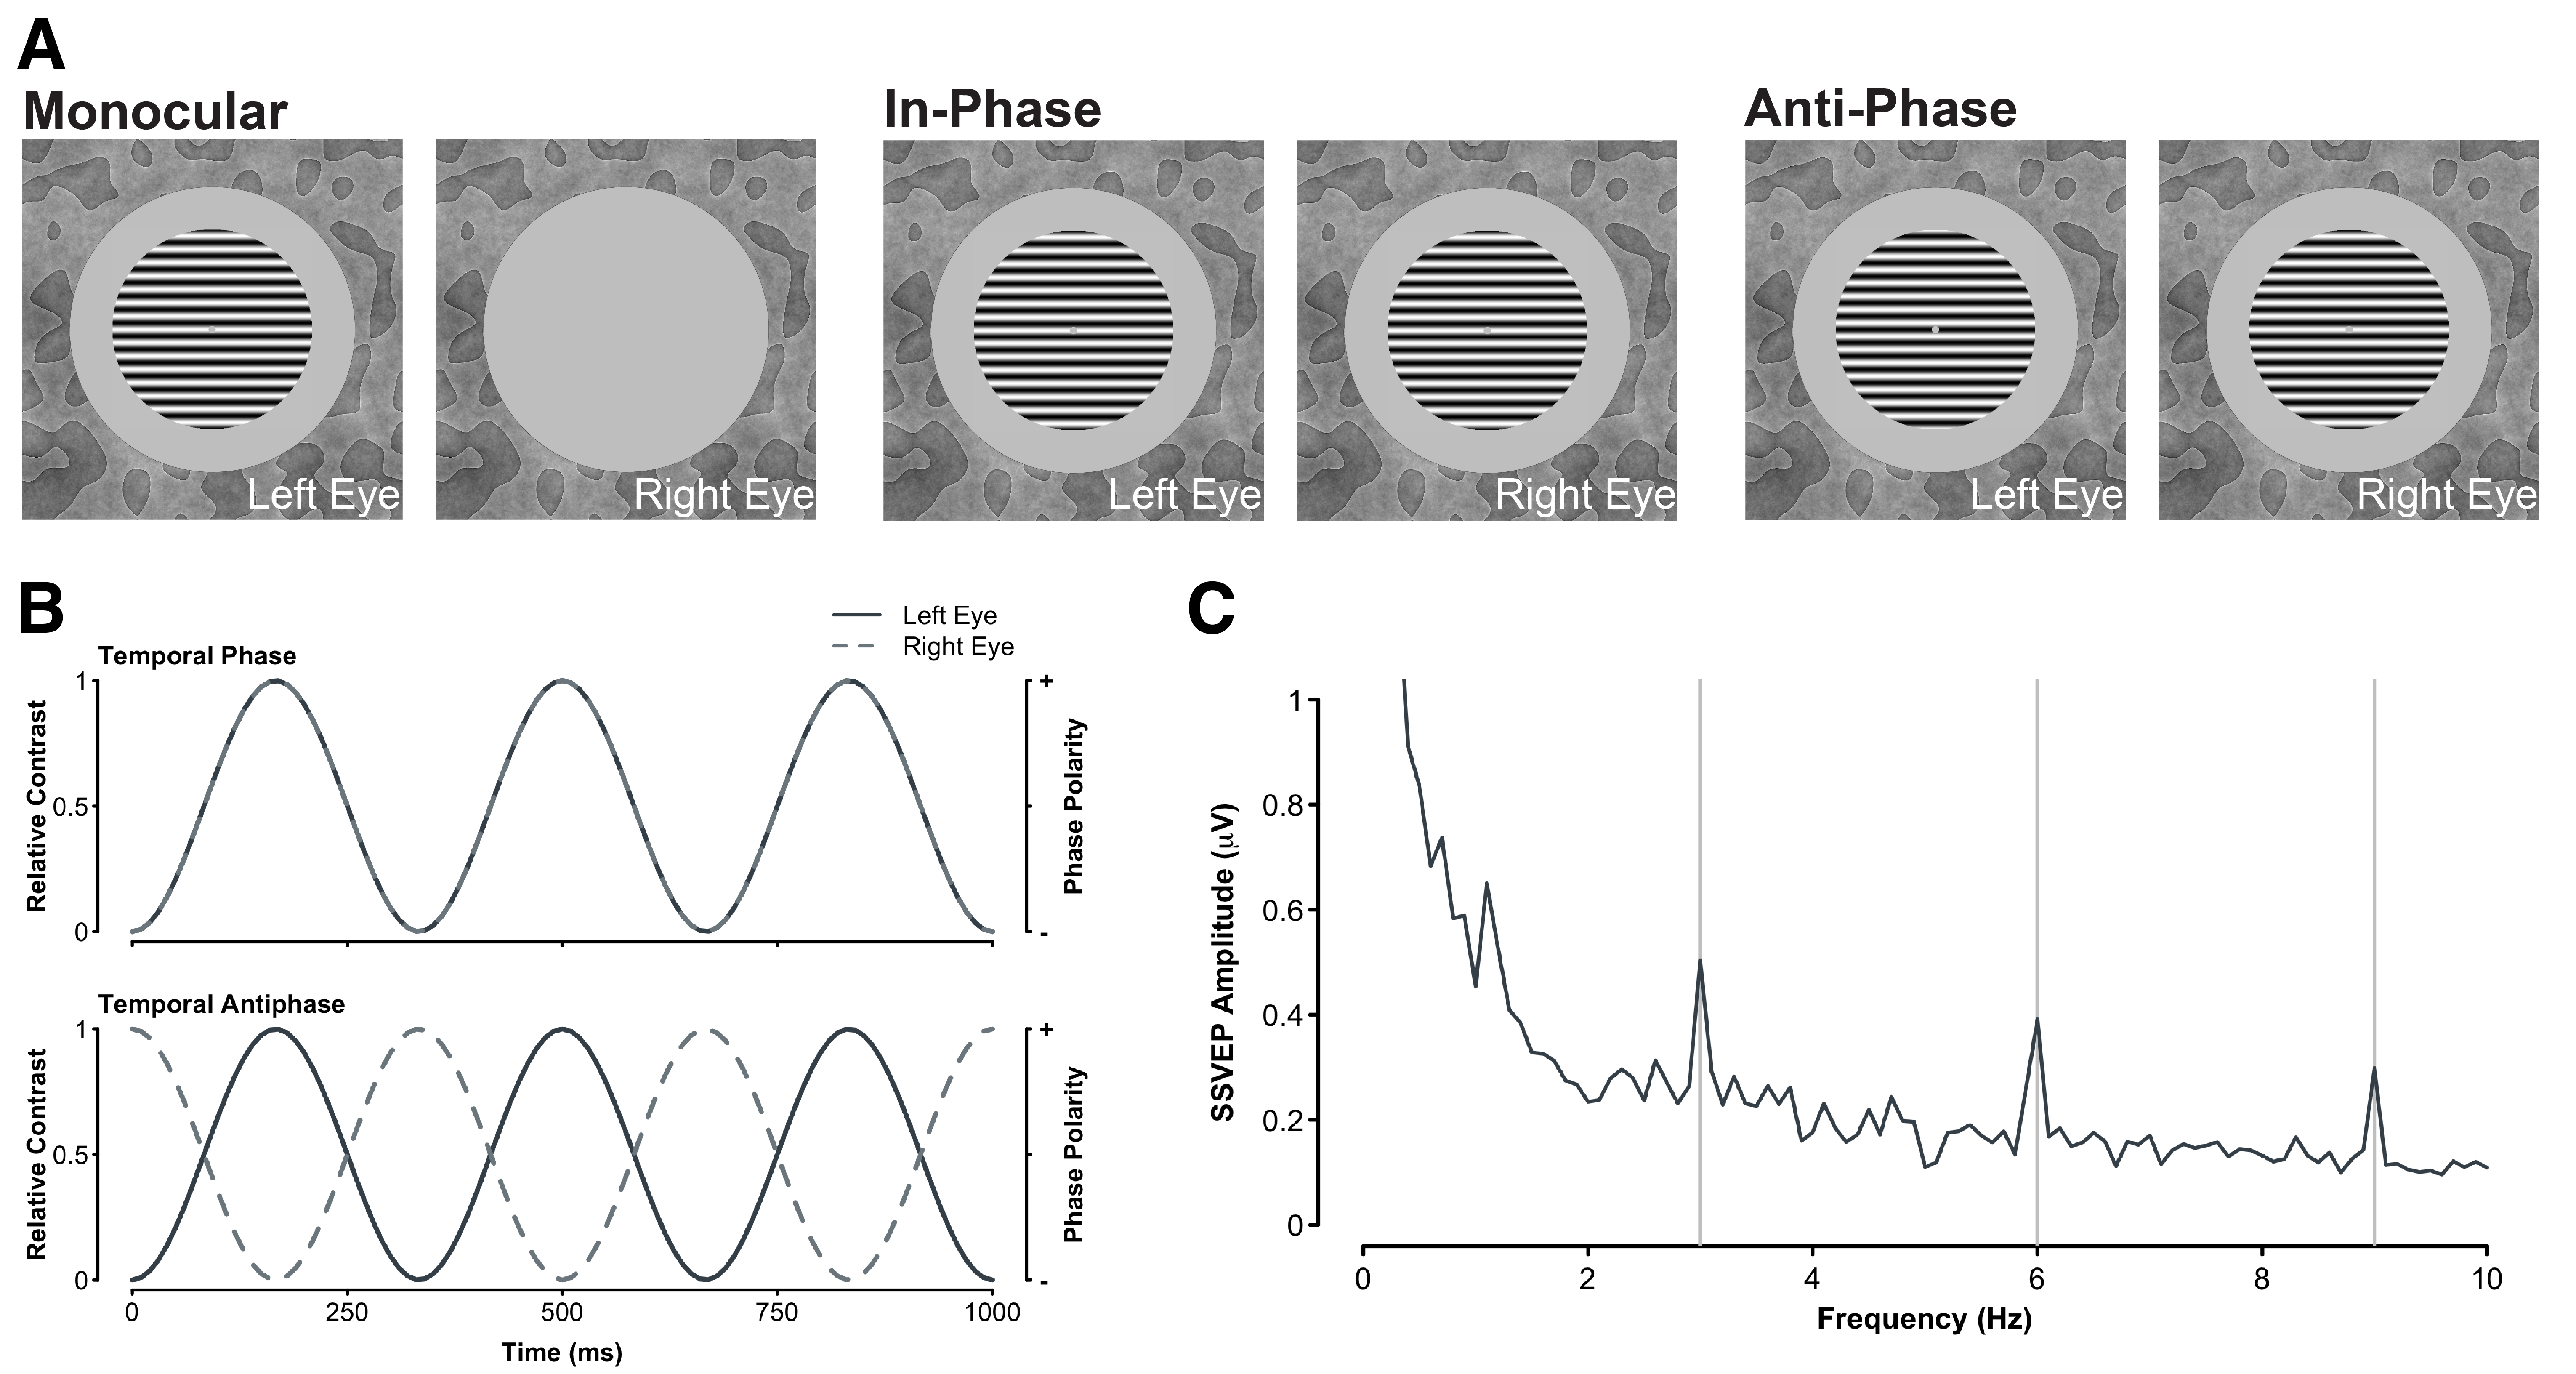
\includegraphics[keepaspectratio]{Figures/MethodsFigure.png}}

}

\caption{\label{fig-methodFigures}\textbf{A}. The spatial configuration
of stimuli presented to observers in our experiment. Monocular
conditions presented the sinusoidal grating to the left or right eye of
observers (counterbalanced) while the other eye was presented with a
gray screen set to mean luminance. Binocular conditions could be shown
with stimuli in spatial phase, whereby the phase of both sinusoidal
gratings was identical, or in spatial anti-phase, where the phase of the
sinusoidal gratings presented to each eye was opposite. The background
texture did not change throughout the trial to aid with binocular
fusion. \textbf{B}. The temporal configuration of our stimuli. To
generate SSVEPs, stimuli were contrast modulated in two ways: on/off
(left Y axis) or counterphase (right Y axis). The oscillatory pattern
could also be in phase (upper plot), where both stimuli were modulated
in the same manner, or in counterphase (lower plot), where as one
stimulus increased in contrast, the other decreased in contrast (or
increased in opposite polarity). \textbf{C}. Example SSVEPs generated
under binocular spatial and temporal in-phase viewing of stimuli for one
observer, averaged across four electrodes (\emph{Oz}, \emph{POz},
\emph{O1}, \emph{O2}) and 12 repetitions.}

\end{figure}%

Observer SSVEPs were measured with a single horizontal sinusoidal
grating that subtended \(15^\circ\) of visual angle on the retina with a
spatial frequency of 3 cycles/\(^\circ\) of visual angle
(Figure~\ref{fig-methodFigures}A). Our experimental conditions modulated
the interocular spatial phase of stimuli
(Figure~\ref{fig-methodFigures}A). Under binocular viewing, the
sinusoidal gratings could be presented in spatial phase or spatial
anti-phase. When stimuli were presented in spatial phase, the aligned
sinusoidal gratings were identical in both eyes (\(\Delta \phi = 0\)).
The spatial anti-phase condition phase-shifted one of the sinusoidal
gratings by 180\(^o\) (\(\Delta \phi = \pi\)). Stimuli were also
modulated in their oscillatory pattern, which could be On/Off or
counterphase flicker at a frequency of 3Hz
(Figure~\ref{fig-methodFigures}B). Under On/Off contrast flicker, the
relative contrast of the gratings began at 0\%, increased smoothly to
100\% of the nominal maximum (100\% Michelson contrast), and then
returned to 0\% over 333 ms (i.e., one cycle). On/Off flicker will
generate SSVEPs at the fundamental frequency (3Hz) and its integer
harmonics (2F, 3F, 4F, see Figure~\ref{fig-methodFigures}C).
Counterphase flicker reversed the phase of the gratings at a frequency
of 3Hz. The contrast of the grating began at the relative maximum
(100\%), gradually decreased to 0\% of the relative maximum, and then
increased again to 100\% but in the opposite phase polarity. Unlike
On/Off flicker, counterphase flicker generates two nearly identical
transients per cycle and thus does not produce SSVEPs at the fundamental
frequency (3Hz) but only its even harmonics (Wade and Baker, 2025).

To aid with binocular fusion, stimuli were surrounded by a static
binocular texture presented beyond the central 19\(^o\) stimulus
aperture. These textures were constructed by first low-pass filtering a
white (amplitude \(\propto 1/f^0\)) noise pattern, dichotomizing its
output into a binary image, and taking its phase spectrum. A second flat
(amplitude \(\propto 1/f^0\)) was adjusted by multiplying each spatial
frequency's amplitude coefficient by \(f^{-1}\) to generate a pink
amplitude spectrum (Hansen and Hess, 2006; Tadmor and Tolhurst, 1994).
The pink amplitude spectrum and the phase spectrum of the binary image
were rendered in the spatial domain by taking the inverse Fourier
transform, resulting in the pattern shown in
Figure~\ref{fig-methodFigures}A.

\subsection{Procedures}\label{procedures}

Steady-State Visually Evoked Potentials (SSVEPs) were recorded with
monocular and binocular stimulation using either on-off or counterphase
flicker at 3Hz. Across the eyes, binocular stimuli could be in spatial
and temporal phases, temporal phase but spatial anti-phase, spatial
phase but temporal anti-phase, or spatial and temporal anti-phase
(on-off flicker only). Stimuli presented in spatial and temporal
anti-phase under counterphase flicker are identical to stimuli presented
in spatial and temporal phase (and so we did not duplicate this
condition). Thus, this experiment was comprised of nine conditions - two
monocular and seven binocular - each repeated 12 times for a total of
108 trials. Stimulus presentation was separated into four experimental
blocks, each containing 27 trials. A trial lasted 15 seconds; a grating
stimulus flickered onscreen for 11 seconds, followed by a screen with
its central 19\(^o\) set to mean luminance for 4 seconds. Participants
completed all 27 trials of an experimental block in a single sequence
(6.75 minutes) and were given breaks between experimental blocks. The
trial order was pseudo-randomized on each block. Participants did not
receive explicit task instructions other than to fixate the marker in
the center of the display and blink only during the blank period between
stimulus presentations.

\subsection{SSVEP Analysis}\label{ssvep-analysis}

We used whole-head average referencing to normalize each electrode to
the mean signal of all 64 electrodes (for each sample point). The EEG
waveforms were Fourier transformed at each electrode for a 10-second
window, beginning one second after the stimulus onset to avoid onset
transients. The Fourier spectra were coherently averaged (i.e.,
retaining the phase information) across four occipital electrodes
(\emph{Oz}, \emph{POz}, \emph{O1}, and \emph{O2}) and trial repetitions
(see Figure~\ref{fig-methodFigures}C). We then calculated
signal-to-noise ratios (SNRs) by dividing the absolute amplitude in the
signal bin (e.g., 3 Hz) by the mean of the absolute value of the ten
adjacent bins (\(\pm 0.5\) Hz in steps of 0.1 Hz). Given that
distributions of ratios (including SNRs) are inherently skewed, the
median SNR was taken across all participants; the median is a more
robust descriptor of central tendency in skewed distributions.

\section{Results}\label{results}

\begin{figure}

\centering{

\pandocbounded{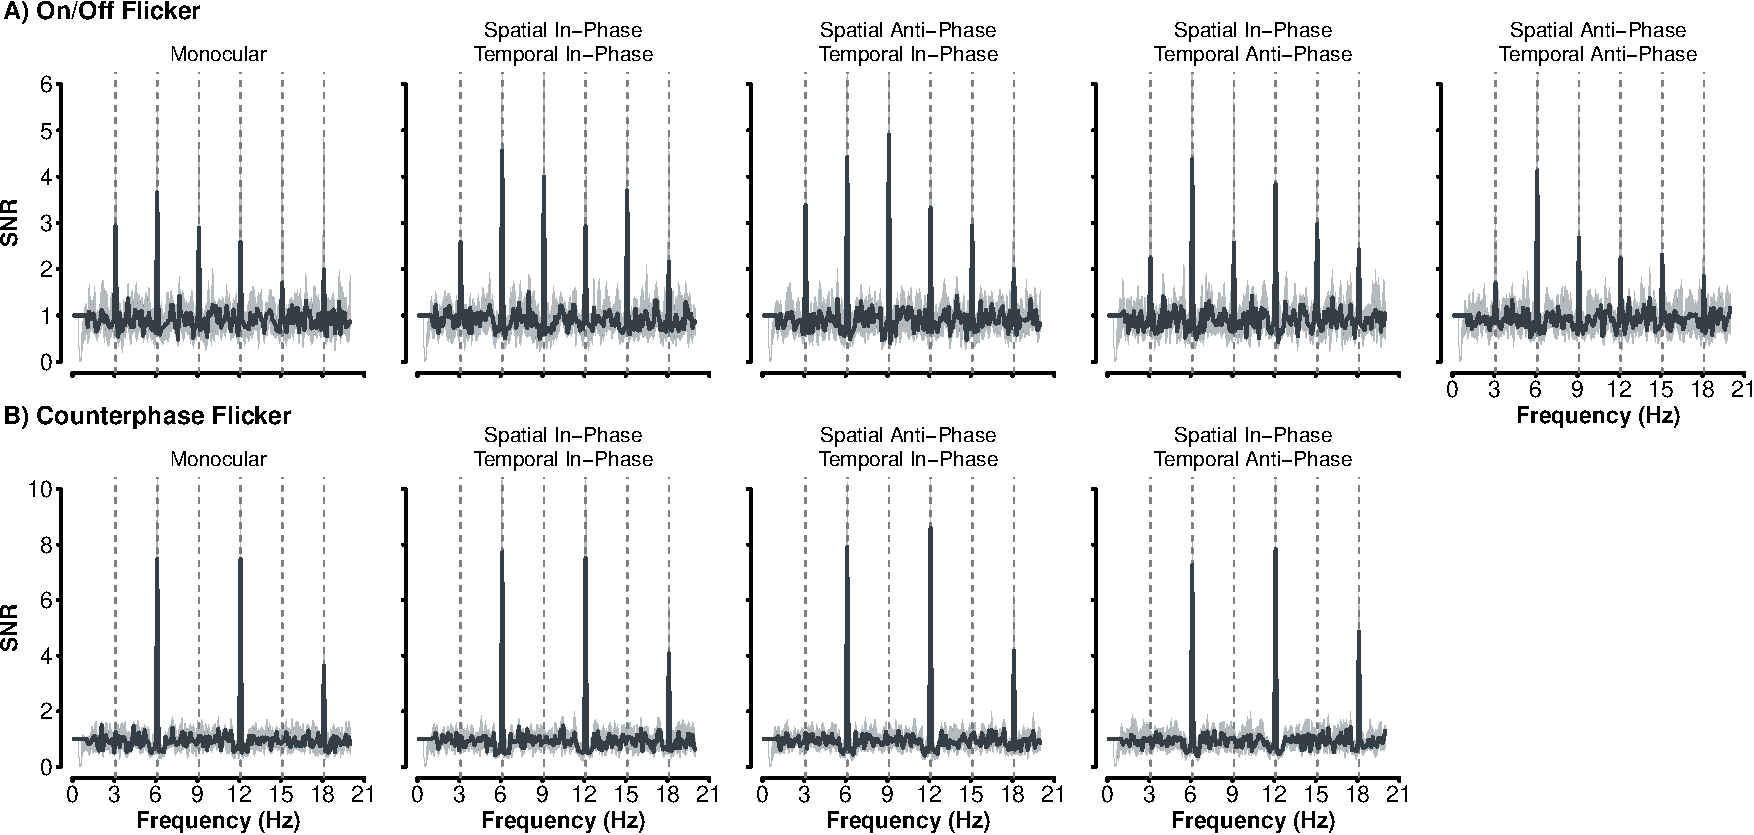
\includegraphics[keepaspectratio]{SSVEP_Phase_AntiPhase_paper_files/figure-pdf/fig-SNRData-1.pdf}}

}

\caption{\label{fig-SNRData}Cross-participant median SNRs for
frequencies up to 20Hz. SNRs generated by On/Off flicker are shown in
the top row (A), while those generated by counterphase flicker are shown
in the bottom row (B). The light gray area represents bootstrapped 95\%
confidence intervals that were calculated by resampling (with
replacement) participant SNRs 2000 times.}

\end{figure}%

Figure~\ref{fig-SNRData} shows the cross-participant median SNR spectra
for all experimental conditions. Responses for all On/Off flicker
experimental conditions generated peaks at the fundamental frequency
(3Hz) and its harmonics (integer multiples of 3Hz). Similarly,
counterphase flicker produced responses at twice the flicker frequency
(6 Hz) and its harmonics. We assessed differences in SNR magnitude
across experimental conditions via a permutation test, allowing a
non-parametric comparison of a statistic between two conditions. We
first take the median difference between two experimental conditions
(i.e., the observed difference) to conduct the permutation tests. A null
distribution is then constructed by combining SNR values from both
experimental conditions, and randomly sampling them without replacement
to create two groups of sizes identical to their original, but with
values not associated with a particular experimental condition. The
median difference of the randomly sampled SNRs is then taken. This
process is repeated multiple times (e.g., \(N =\) 2000 iterations) to
build a distribution of median differences with no association of
experimental condition (i.e., a null-hypothesis distribution). The
observed median difference is then compared to this distribution. The
proportion of scores greater than the observed difference represents the
\(p\) value associated with the test. When comparing SNRs at the
fundamental frequency (3Hz) for On/Off flicker, we find no statistically
significant difference in median SNR magnitude between experimental
conditions where stimuli were presented in temporal phase (see
Figure~\ref{fig-SNRComparison}). Monocular and binocular presentation
for stimuli presented in temporal phase resulted in a similar response
pattern under both On/Off and counterphase flicker modulations. This is
consistent with ocularity invariance; binocular and monocular stimuli
appear equal in magnitude at high contrast (Baker et al., 2007a; Meese
et al., 2006).

\begin{figure}

\centering{

\pandocbounded{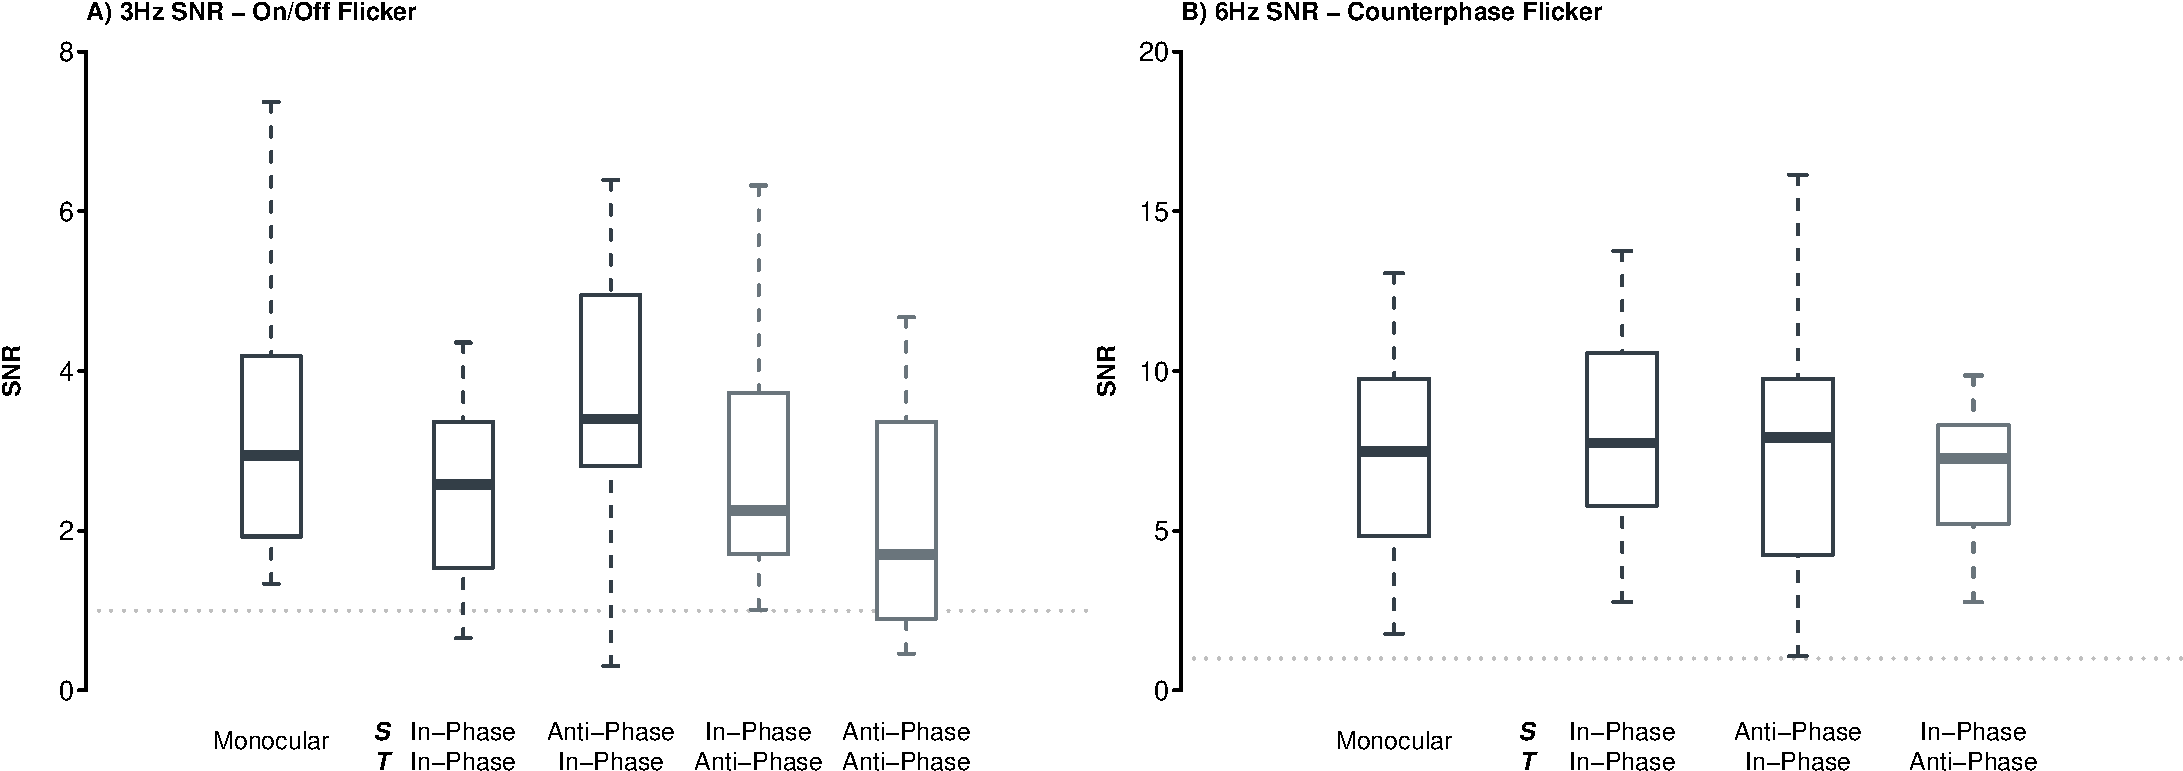
\includegraphics[keepaspectratio]{SSVEP_Phase_AntiPhase_paper_files/figure-pdf/fig-SNRComparison-1.pdf}}

}

\caption{\label{fig-SNRComparison}Boxplots of participant SNRs at the
fundamental frequency for each experimental condition in our study. A)
Boxplots represent the participant SNR at 3Hz. The median SNR is shown
by the thick line within the box, with the lower and upper border of the
box representing the first (25\%) and third (75\%) quartile of the SNR
distribution. Dashed lines show the lower and upper whisker limits,
which are calculated as 1.5 times the interquartile range (distance
between the third and first quartile). Boxplots for the binocular
conditions have labels for their spatial (S) and temporal (T) phase
relationships. Experimental conditions where stimuli are presented in
temporal anti-phase are shown in a lighter gray. B) As in A, boxplots
show participant SNRs at 6Hz, the fundamental frequency for counterphase
flicker. In both graphs, the dashed line represents an SNR of 1.0.}

\end{figure}%

Changing the phase relationships of stimuli under On/Off flicker had
some interesting impacts on the fundamental frequency
(Figure~\ref{fig-SNRComparison}A). Stimuli presented in spatial phase
and temporal anti-phase generated smaller SNRs (median\(_{\text{SNR}}\)
= 2.25) than stimuli presented in spatial anti-phase and temporal phase
(median\(_\text{SNR}\) = 3.4, \(p\) = .047). The reduction in the
amplitude relative to stimuli in spatial anti-phase and temporal phase
was also observed for stimuli in temporal and spatial anti-phase
(median\(_\text{SNR}\) = 1.7; \(p\) = .023). No other statistically
significant difference in median SNRs were observed for all counterphase
flicker conditions or the other harmonics for On/Off flicker (all \(p\)
values were greater than .05). While the median SNRs under On/Off
flicker shown in temporal anti-phase were reduced in comparison to other
conditions, both the spatial in phase temporal anti-phase condition
(\(p < .001\)) and the spatial and temporal anti-phase conditions
(\(p = .004\)) had median SNR values that were statistically
significantly greater than 1.0. The presence of a 3Hz response for
binocular stimuli presented in temporal anti-phase indicates that
monocular responses remain and contribute to the SSVEP, as these
conditions generate two transients per cycle and a purely binocular
signal would only generate responses at 6Hz (Blake et al., 1981;
Georgeson et al., 2016; Moulden, 1980).

\subsection{Modelling}\label{modelling}

The perception of binocular stimulus contrast is well-explained by
psychophysical models that process input contrast in two sequential
contrast gain control stages interposed by binocular summation (Baker et
al., 2008, 2007a, 2007b; Baker and Meese, 2007; Meese et al., 2006).
This simple, yet powerful, family of models not only captures
behavioural data well, but can also explain neural responses to
binocular and dichoptic stimuli (Baker and Wade, 2017; Lygo et al.,
2021; Richard et al., 2018). Our SSVEP results show the expected pattern
of binocular combination for stimuli presented at high contrast (i.e.,
ocularity invariance) but also intriguing effects that are likely
explainable by the most recent extension of the two-stage contrast gain
control model, as defined by Georgeson et al. (2016). To explore the
architecture required to describe our effects adequately, we
progressively increase the complexity of binocular combination,
beginning with a deliberately wrong model (i.e., linear combination) and
building up to a multi-channel model with monocular, binocular, and
phase-selective pathways (Figure~\ref{fig-modelDiagram}).

\begin{figure}

\centering{

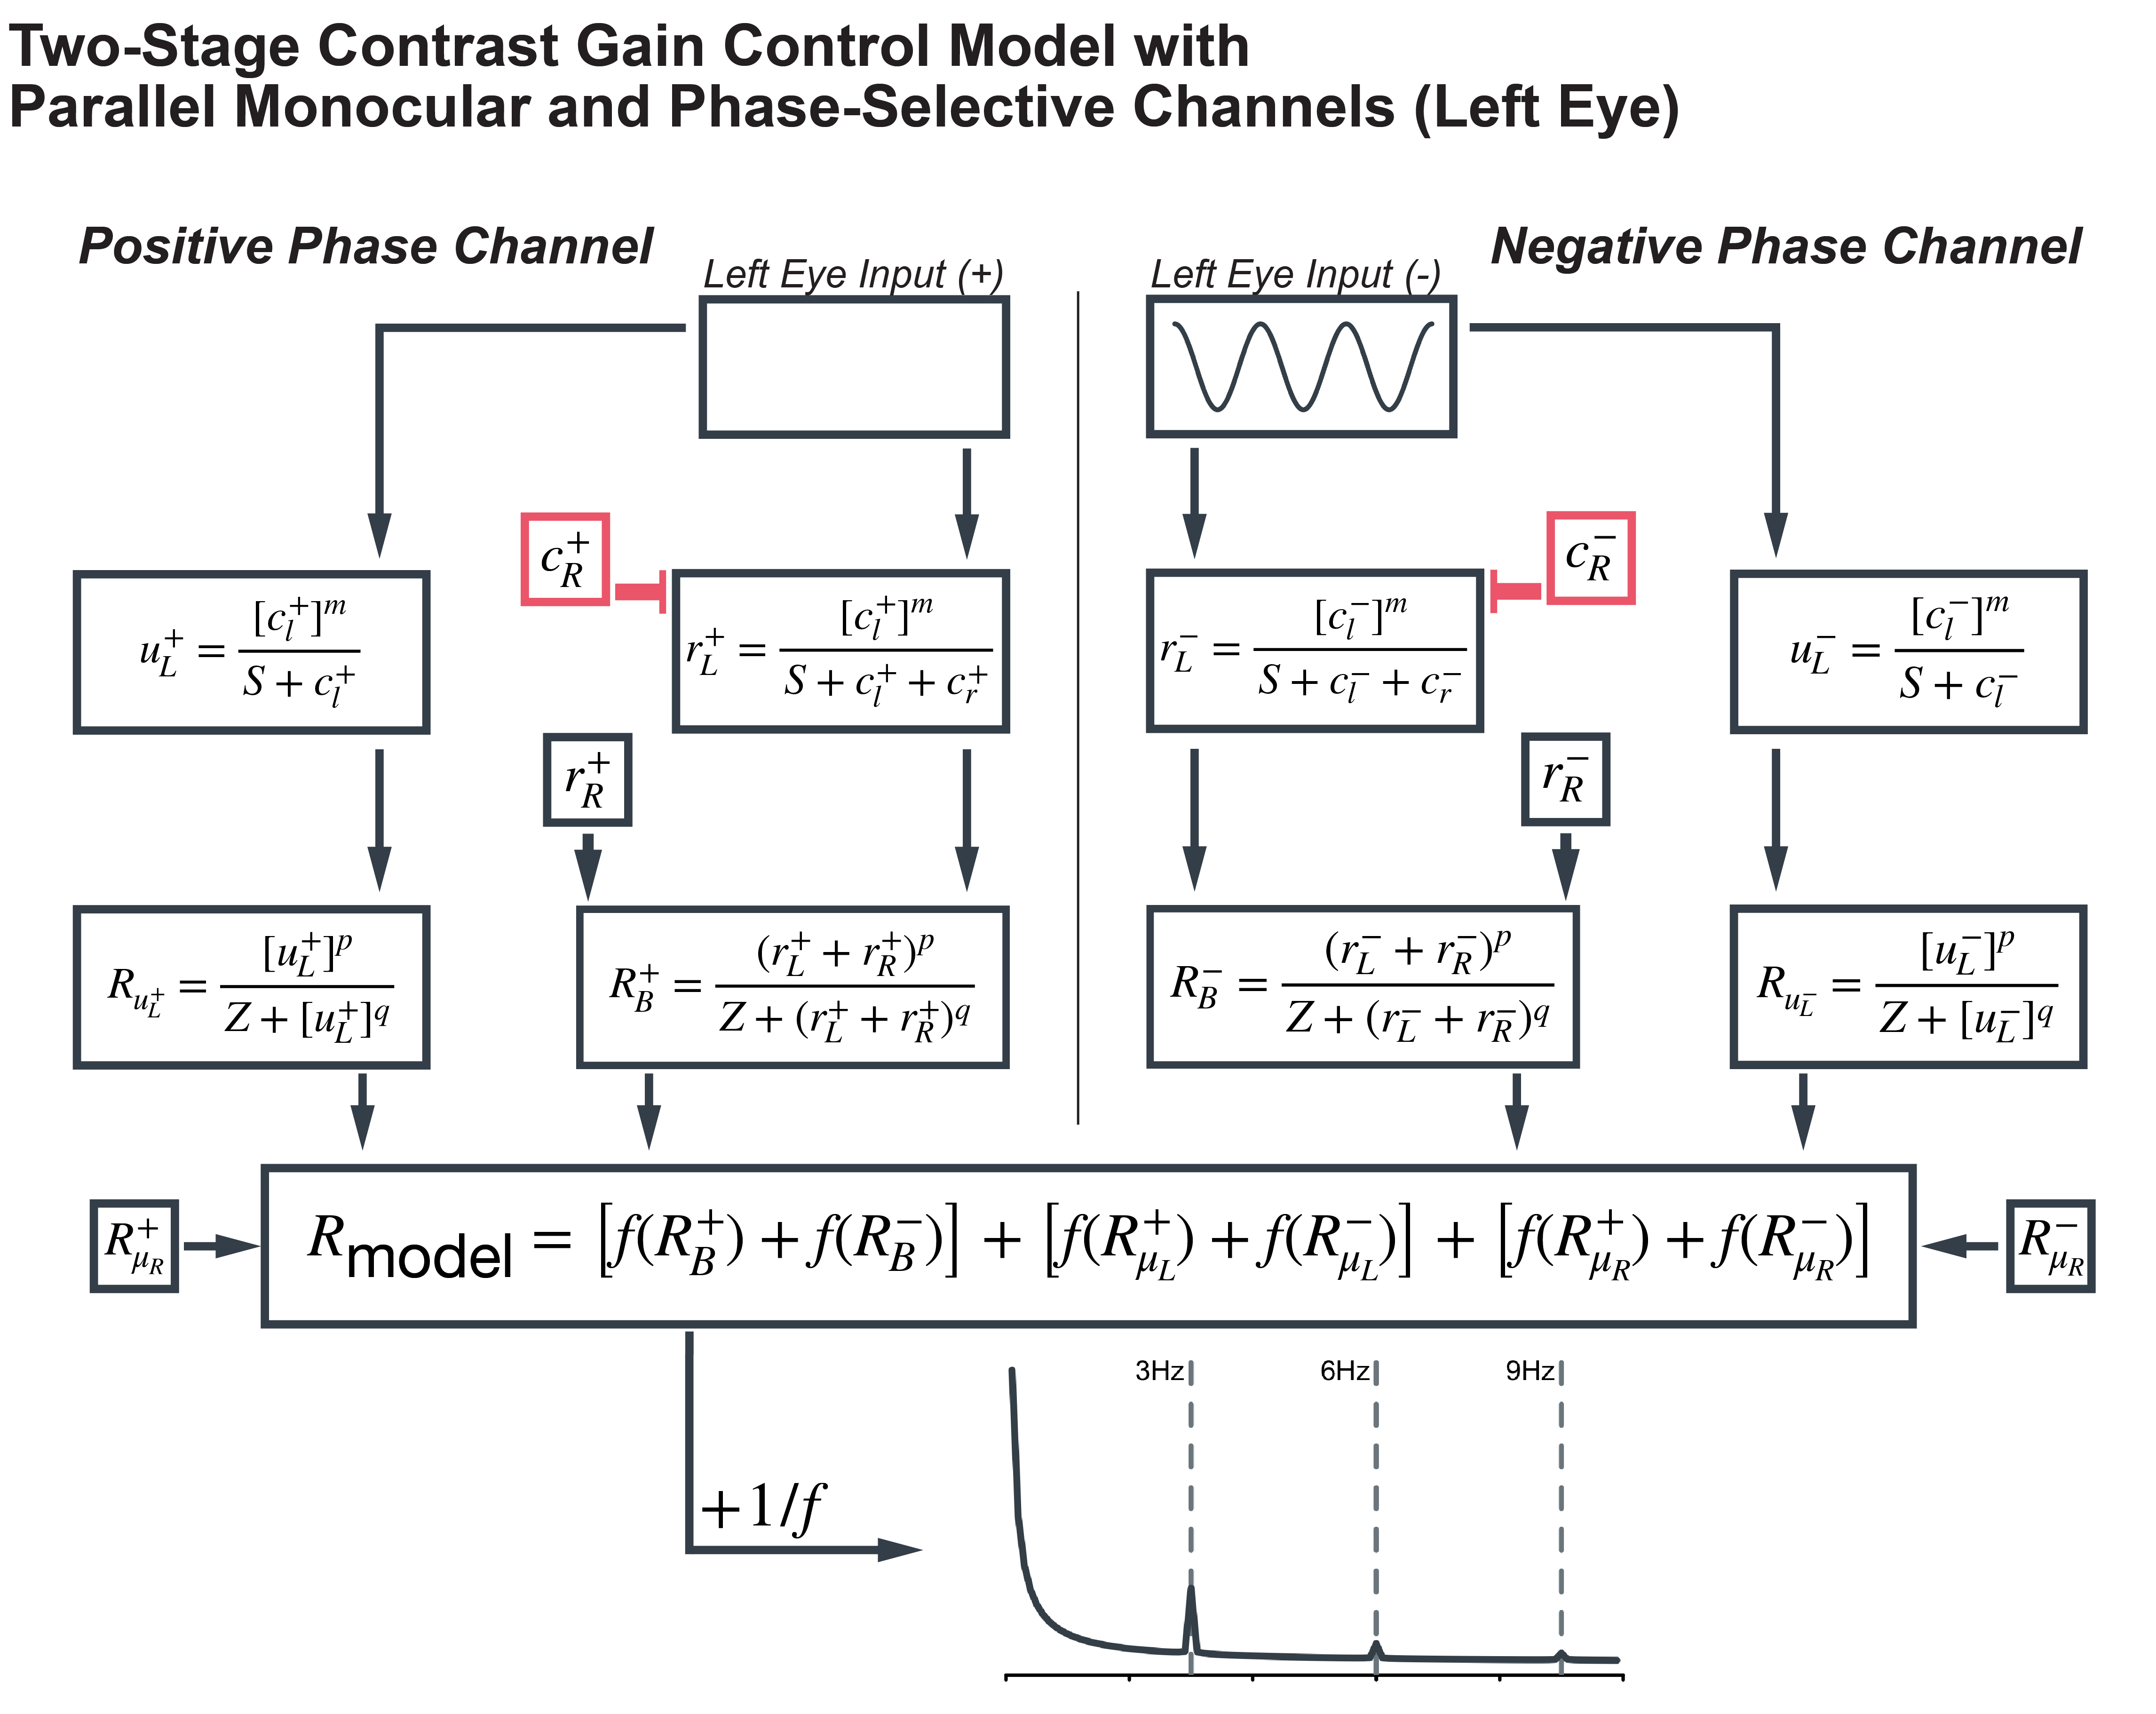
\includegraphics[width=0.8\linewidth,height=\textheight,keepaspectratio]{Figures/FullModel.png}

}

\caption{\label{fig-modelDiagram}This diagram shows the most complex
model variant explored here: the phase-selective two-stage contrast gain
control model with parallel monocular channels. This diagram only shows
the channels for the left eye. Contributions from the right eye
(\(c^+_R\) and \(r^+_R\)) to the binocular channels are shown in small
boxes. Unlike the model defined by Georgeson et al. (2016), responses
from the parallel monocular channels are added to those of the binocular
channels before signal selection for phase-selective channels. This
change accounts for methodological differences when fitting neuroimaging
data. A pink noise spectrum was added to allow for a comparable
calculation of model SNRs as is done with human data.}

\end{figure}%

The architecture of the models explored differs, but all received the
same input and had their final outputs processed identically. The input
to all models was a 3 Hz sine wave, adjusted to accurately represent the
various experimental conditions of this study (see
Figure~\ref{fig-methodFigures}). For example, stimuli presented with an
On/Off flicker in temporal anti-phase had the left eye input generated
by the following equation,
\begin{equation}\phantomsection\label{eq-stimInput2L}{
c_L = A * (\cos(2 \pi ft)+1)/2,
}\end{equation} while the right eye input is defined as,
\begin{equation}\phantomsection\label{eq-stimInput2R}{
c_R = A * (-\cos(2 \pi ft)+1)/2.
}\end{equation} \(A\) represents stimulus contrast (amplitude), \(f\)
the temporal flicker frequency (i.e., 3 Hz), and \(t\) time in
milliseconds. The input to the right eye (\(c_R\)) is phase shifted by
180\(^o\), which is accomplished using the negative cosine function
(\(-cos\)). Finally, sine waves are rectified to the range between 0 and
1 to represent the relative contrast presented to observers. The same
experimental condition with counterphase flicker has the following
sinusoidal profile for the left eye,
\begin{equation}\phantomsection\label{eq-stimInput3L}{
c_L = A * [\cos(2 \pi ft)]_+
}\end{equation} and for the right eye,
\begin{equation}\phantomsection\label{eq-stimInput3R}{
c_R = A * [-\cos(2 \pi ft)]_+.
}\end{equation} These profiles are identical to the On/Off flicker, but
the sine waves are half-wave rectified to represent the counterphase
oscillation. To fit model outputs (rectified sine waves) to observer
data, the final response of the models was Fast Fourier Transformed, and
a pink noise spectrum was added to the Fourier amplitudes,
\(|FFT(R_\text{model})|+1/f\) to simulate neural noise (see e.g.
Donoghue et al., 2020), before calculating model SNRs. All models
developed in this study were fit by minimizing the sum of squared errors
between the model output and the observer median SNRs for the first 6
SSVEP components (3Hz, 6Hz, 9Hz, 12Hz, 15Hz, and 18Hz).

\subsubsection{Evidently wrong models}\label{evidently-wrong-models}

As a first step in defining the necessary architecture to capture our
results, we built baseline models with no monocular stage or phase
selectivity that we do not expect to explain all of our effects. The
first is a purely linear summation model of binocular combination;
\begin{equation}\phantomsection\label{eq-linearSumModel}{
R_B = c_L+c_R,
}\end{equation} the binocular response (\(R_B\)) is the sum of the
monocular inputs. The fits of the linear summation model are shown in
Figure~\ref{fig-badModels1} and its performance metrics in
Table~\ref{tbl-R2Table}. For On/Off flicker, the linear summation model
only generates responses at the fundamental frequency (3Hz) that grossly
overestimate observer SNRs. This is expected as this model lacks the
rectification and non-linearities required to generate responses at the
harmonics (Regan and Regan, 1988; Wade and Baker, 2025). In a linear
sum, stimuli presented under On/Off flicker in temporal anti-phase
cancel each other, and thus the model generates no response. The model
does generate responses at the fundamental and harmonics of the
counterphase flicker condition (Figure~\ref{fig-badModels1}B), but this
is attributable to the input's rectification (the half-wave
rectification applied to the input;
Equation~\ref{eq-stimInput3L}, Equation~\ref{eq-stimInput3R}) and not
the model architecture.

\begin{longtable}[]{@{}
  >{\raggedright\arraybackslash}p{(\linewidth - 6\tabcolsep) * \real{0.5000}}
  >{\centering\arraybackslash}p{(\linewidth - 6\tabcolsep) * \real{0.1667}}
  >{\centering\arraybackslash}p{(\linewidth - 6\tabcolsep) * \real{0.1667}}
  >{\centering\arraybackslash}p{(\linewidth - 6\tabcolsep) * \real{0.1667}}@{}}
\toprule\noalign{}
\begin{minipage}[b]{\linewidth}\raggedright
Model
\end{minipage} & \begin{minipage}[b]{\linewidth}\centering
\(R^2\)
\end{minipage} & \begin{minipage}[b]{\linewidth}\centering
RMSE
\end{minipage} & \begin{minipage}[b]{\linewidth}\centering
AIC
\end{minipage} \\
\midrule\noalign{}
\endfirsthead
\toprule\noalign{}
\begin{minipage}[b]{\linewidth}\raggedright
Model
\end{minipage} & \begin{minipage}[b]{\linewidth}\centering
\(R^2\)
\end{minipage} & \begin{minipage}[b]{\linewidth}\centering
RMSE
\end{minipage} & \begin{minipage}[b]{\linewidth}\centering
AIC
\end{minipage} \\
\midrule\noalign{}
\endhead
\bottomrule\noalign{}
\tabularnewline
\caption{Goodness-of-fit metrics for all models compared in this study.
Errors in predictions for the linear sum model were too large to
calculate \(R^2\). RMSE is the Root Mean Square error and AIC is the
Aikaike Information Criterion.}\label{tbl-R2Table}\tabularnewline
\endlastfoot
Linear sum & - & 3.234 & 281.99 \\
Linear sum, with Rectification & 0.575 & 1.405 & 197.95 \\
Two-Stage, no interocular interactions & 0.822 & 0.908 & 154.86 \\
Two-Stage, with interocular interactions & 0.81 & 0.94 & 158.62 \\
Two-Stage with parallel monocular channels & 0.877 & 0.756 & 135.1 \\
Two-Stage with phase-selective channels \& monocular channels & 0.876 &
0.759 & 135.39 \\
\end{longtable}

Responses of neurons to contrast in the visual system are well-modeled
by a saturating non-linearity: as contrast increases, the magnitude of
responses saturates (the rise in response per unit contrast decreases at
higher contrast values (Heeger, 1992)). The saturating non-linearity can
be modeled in different ways, but generally contains a divisive
suppression and an exponentiation of the excitatory and inhibitory
inputs. Including suppression can aid the model in better capturing the
magnitude of responses in our observers, while exponents introduce the
non-linearities required to generate responses at the harmonic
frequencies. Thus, the next increment of model complexity defines the
binocular response as the contrast gain control equation (after Legge,
1984b): \begin{equation}\phantomsection\label{eq-firstBinocSum}{
R_B = \frac{(c_L+c_R)^p}{Z+(c_L+c_R)^q},
}\end{equation} where the binocular response of the model (\(R_B\)) is
defined as the sum of monocular inputs (\(c_L\) and \(c_R\)) raised to
the power \(p\) normalized by the sum of monocular inputs raised to the
power \(q\) and where (\(p\) \textgreater{} \(q\)). The parameter Z
prevents division by zero and sets overall sensitivity. The model can
now generate responses at the harmonic frequencies for stimuli presented
in temporal phase under On/Off flicker (see Figure~\ref{fig-badModels1}
and Table~\ref{tbl-R2Table}). While this model iteration improves on the
fits, it nevertheless struggles to fit SNR values at the fundamental
frequency (3Hz) and is, as with the linear summation model, incapable of
generating responses to stimuli presented with On/Off flicker in
temporal anti-phase; the linear sum of stimuli presented in temporal
anti-phase will always return zero. Therefore, the model still lacks the
necessary architecture to define neural responses to our stimuli
adequately.

\begin{figure}

\centering{

\pandocbounded{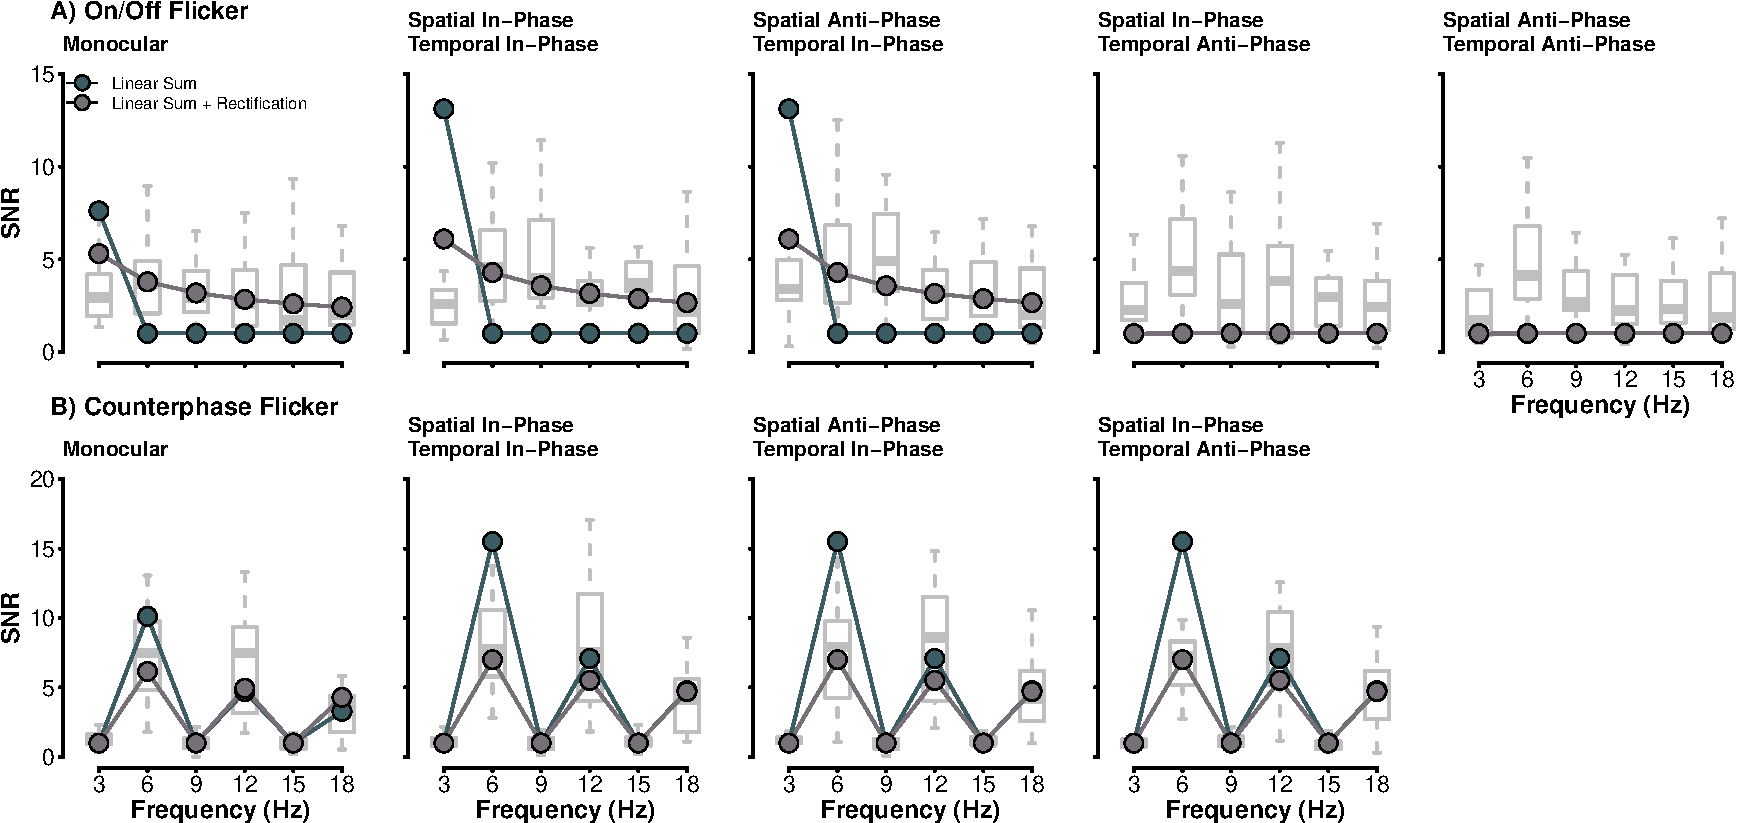
\includegraphics[keepaspectratio]{SSVEP_Phase_AntiPhase_paper_files/figure-pdf/fig-badModels1-1.pdf}}

}

\caption{\label{fig-badModels1}Fits of the linear sum (green) and the
rectified linear sum (brown) models. Boxplots behind model responses
show the distribution of observer SNRs. Model SNRs were fit to the
median SNR of observers, which is represented by the thicker line within
each box.}

\end{figure}%

\subsubsection{The Two-Stage Contrast Gain Control
Model}\label{the-two-stage-contrast-gain-control-model}

The simple models described above could not accurately represent the
observer SSVEPs we recorded. They overestimated SNRs at the fundamental
frequency and failed to generate responses for stimuli presented in
temporal anti-phase with On/Off flicker. A potential model refinement is
adding a monocular transducer before binocular combination (Meese et
al., 2006). The architecture of this model now begins with a monocular
stage \begin{equation}\phantomsection\label{eq-firstStageofTwoNoInter}{
r_L = \frac{c_L^m}{S + c_L}, \qquad r_R = \frac{c_R^m}{S + c_R}
}\end{equation} where an exponent (\(m\)) is applied to the monocular
inputs (\(c_L\) and \(c_R\)) in addition to self-suppression. The
outputs of the monocular stage are then fed into a binocular stage that
undergoes a second contrast gain control,
\begin{equation}\phantomsection\label{eq-binocComb}{
R_{B} = \frac{(r_L+r_R)^p}{Z+(r_L+r_R)^q}.
}\end{equation} In this model variant, \(m\) is the monocular exponent
that determines the extent of summation at detection threshold, with
moderation by the suppressive term. In the second stage, \(p > q\) as
with Equation~\ref{eq-firstBinocSum}, which is necessary to capture the
mild facilitatory effects of dichoptic masking (Meese et al., 2006), and
determines the shape of contrast discrimination functions. We can
strengthen the normalization of the monocular input by adding
interocular suppression and replacing
Equation~\ref{eq-firstStageofTwoNoInter} (the first stage) with:
\begin{equation}\phantomsection\label{eq-firstStageofTwo}{
r_{L} = \frac{c_L^m}{S + c_L + c_R}, \qquad r_R = \frac{c_R^m}{S + c_R + c_L}.
}\end{equation} This model iteration is identical to the two-stage
contrast gain control model defined by Meese et al. (2006).

\begin{figure}

\centering{

\pandocbounded{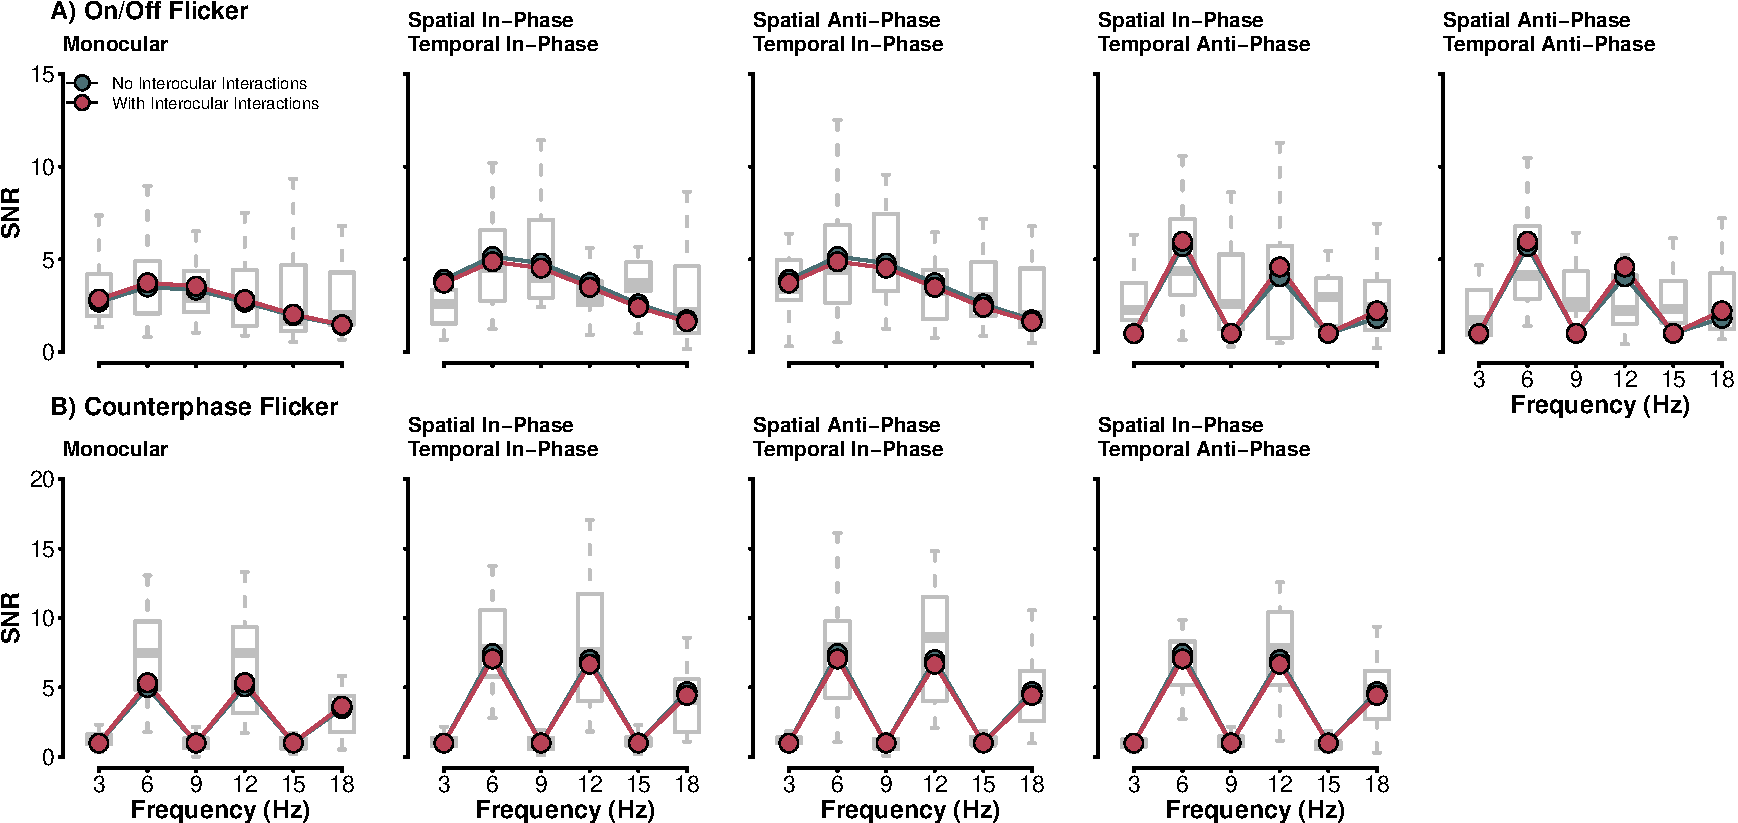
\includegraphics[keepaspectratio]{SSVEP_Phase_AntiPhase_paper_files/figure-pdf/fig-betterModels-1.pdf}}

}

\caption{\label{fig-betterModels}Fits of the two-stage contrast gain
control model without (green) and with (red) interocular suppression.
Boxplots behind model responses show the distribution of observer SNRs.
Model SNRs were fit to the median SNR of observers, which is represented
by the thicker line within each box.}

\end{figure}%

The fits of both model variants, with and without interocular
suppression, are shown in Figure~\ref{fig-betterModels}. The difference
in their quality is negligible (see Table~\ref{tbl-R2Table}) as both
describe most experimental conditions well. The addition of the
monocular transducer enables the model to fit observer SNRs at the
fundamental frequency for stimuli presented in temporal phase under
On/Off flicker, and importantly, it now generates responses for stimuli
presented in temporal anti-phase. The transduced monocular inputs no
longer cancel each other at the binocular stage. While the model can
create responses to temporal anti-phase stimuli, it only does so at the
even harmonics (2F-6Hz, 4F-12Hz, and 6F-18Hz) of the SSVEP spectrum.
This is expected as the model can only generate binocular responses; it
does not preserve monocular signals beyond the first stage. As the two
rectified sine waves are in anti-phase, their sum will generate a new
waveform with frequencies twice the original (6Hz) frequency and its
integer harmonics (2F-12Hz and 3F-18Hz). The responses we recorded at
the fundamental frequency (3Hz) and its odd integer harmonics (3F - 9Hz,
5F - 15Hz) cannot be explained by an architecture with a purely
binocular output. Next, we explore methods of preserving the monocular
signal to explain observer responses to stimuli presented in temporal
anti-phase.

\subsubsection{Parallel Monocular and Phase-Selective
Channels}\label{parallel-monocular-and-phase-selective-channels}

Based on the models described above, observer SSVEPs for stimuli
presented in temporal anti-phase imply the presence of both a binocular
and monocular response in the population response. To preserve the
monocular response in the modelling, we add parallel monocular channels
to the two-stage contrast gain control model, similar to Georgeson et
al. (2016). These channels are fully monocular and do not include
interocular suppression,
\begin{equation}\phantomsection\label{eq-monocFirstStage}{
\mu_L = \frac{C_L^m}{S + C_L}, \qquad  \mu_R = \frac{C_R^m}{S + C_R}.
}\end{equation} In this equation, \(\mu_L\) is the output of the left
eye's first stage of the monocular channel, and \(\mu_R\) is that of the
right eye. The excitatory exponent \(m\) is identical to the channels
that include binocular interaction (see
Equation~\ref{eq-firstStageofTwo}). The output of the monocular channels
undergoes a second contrast gain control stage similar to that of the
binocular channel,
\begin{equation}\phantomsection\label{eq-monocSecondStage}{
R_{\mu_L} = \frac{\mu_L^p}{Z + \mu_L^q}, \qquad  R_{\mu_R} = \frac{\mu_R^p}{Z + \mu_R^q}.
}\end{equation} \(R_{\mu_L}\) and \(R_{\mu_R}\) represent the final
responses of the left and right monocular channels. No additional free
parameters are included in the model with parallel monocular channels;
the parameters \(m\), \(p\), \(q\), \(S\), and \(Z\) used to define the
monocular channel responses are identical to those of the binocular
channels.

The inclusion of parallel monocular channels poses an interesting
problem in our modelling as we now contend with three visual cues from
which to generate model SSVEPs: monocular left (\(R_L\)), monocular
right (\(R_R\)), and binocular (\(R_B\)). Psychophysically, cue
selection has been implemented as a Minkowski sum with a large
(\(\approx 30\)) exponent (Georgeson et al., 2016), approximating a MAX
rule. This method is inappropriate when modelling neural data, as the
recordings from the scalp represent an amalgamation of all responses
generated by the stimuli (Wade and Baker, 2025). Our model output must
therefore represent the combination of signals instead of the selection
of the strongest signal. Here, it is implemented as the sum of the
Fourier amplitude spectra of all three channel outputs. This sum
preserves the amplitude responses required to generate SSVEPs and
prevents the nullifying of responses from summing signals in anti-phase.

Preserving monocular responses until the output stage with parallel
monocular channels improved the fit to our data (see
Table~\ref{tbl-R2Table} and Figure~\ref{fig-bestModels}). The model now
captures responses at the fundamental (3Hz) and odd-integer harmonics
(9Hz and 15Hz) of the temporal anti-phase conditions under On/Off
flicker. Monocular signals, while weaker than binocular signals, are
preserved in the neural responses of observers and thus must be
accounted for in their computational description. As proposed by
Georgeson et al. (2016), parallel monocular channels appear to be an
adequate descriptor of monocular signals.

\begin{figure}

\centering{

\pandocbounded{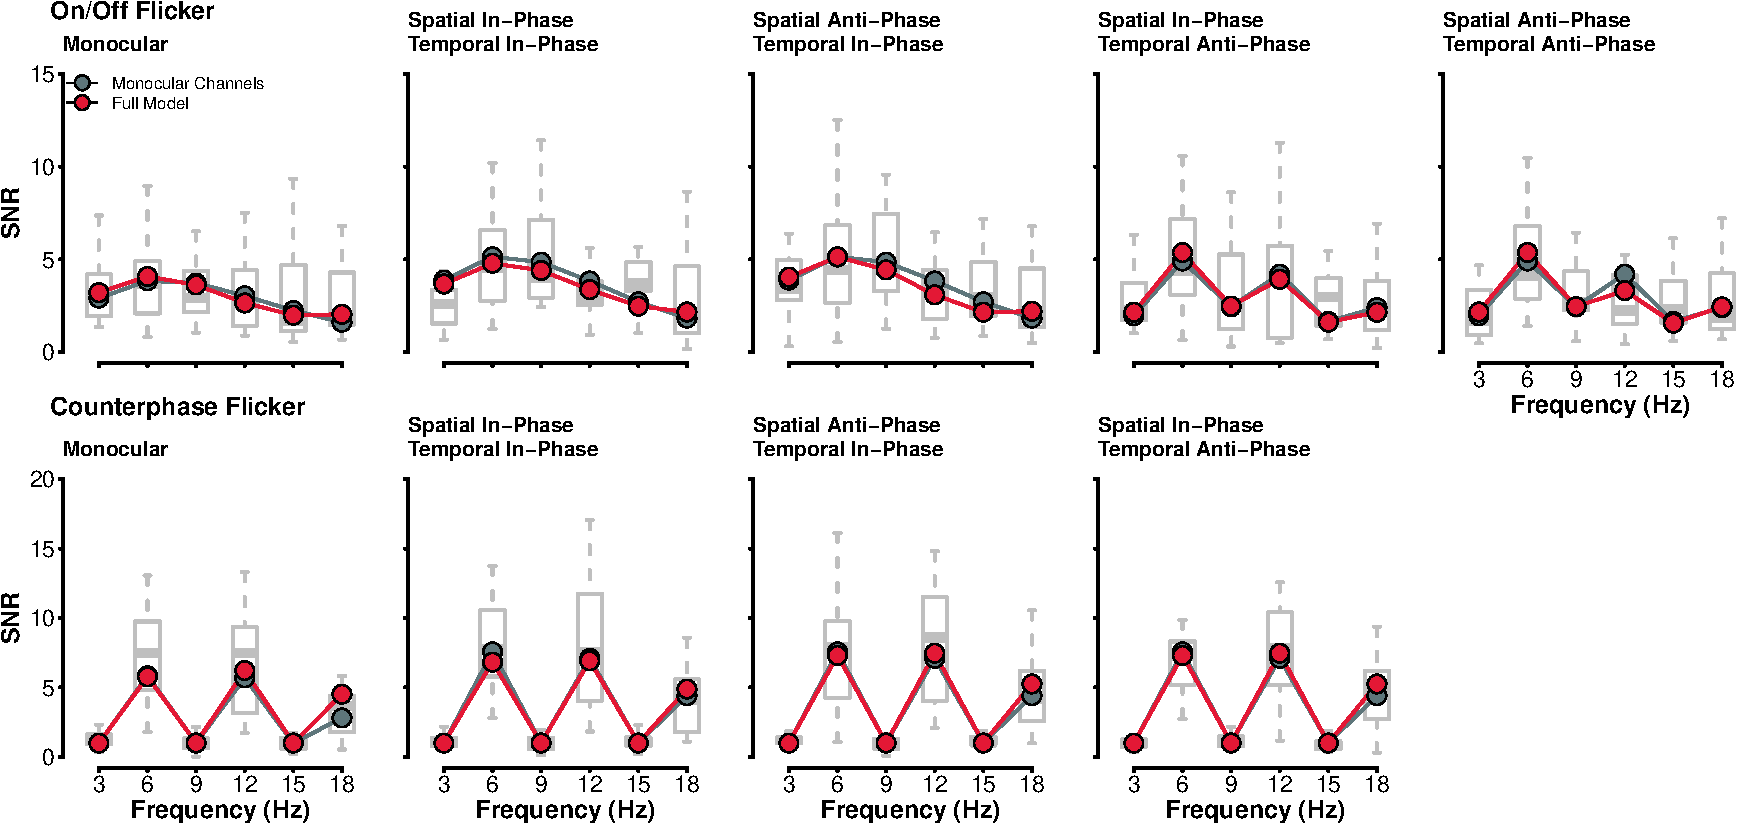
\includegraphics[keepaspectratio]{SSVEP_Phase_AntiPhase_paper_files/figure-pdf/fig-bestModels-1.pdf}}

}

\caption{\label{fig-bestModels}Fits of the two best performing models to
our observer data. Both models, that including parallel monocular
channels and the full model with the added phase-selective channels
perform quite similarly.}

\end{figure}%

Psychophysically, spatial phase has a meaningful impact on binocular
combination (Bacon, 1976; Baker and Meese, 2007; Simmons, 2005) and the
two-stage contrast gain control often includes phase-selective channels
to account for these effects. Our study found little evidence of any
influence of spatial phase on observer SSVEPs, as no statistically
significant difference in signal-to-noise ratios across spatial phase
was found. Still, we felt it prudent to verify if adding phase-selective
channels improves the fit of the model to our data. Phase-selectivity
was added to the binocular and monocular channels by replicating the
equations of the first and second stage, for six channels (see
Figure~\ref{fig-modelDiagram}). As with the previous model, no
additional model parameters were required to include phase-selectivity;
the parameters \(m\), \(p\), \(q\), \(S\), and \(Z\) were used to define
the responses of all six channels in this model.

Model responses were generated from sine waves (in temporal phase or
anti-phase) fed into their respective positive or negative phase
channels. This simulated the spatial phase of stimuli presented to
observers. We refer to this model iteration as the full model, as it
includes a binocular channel with a monocular stage (with interocular
interactions), a binocular stage, parallel monocular channels (with
their respective stages), and phase-selectivity. This is, in essence,
the 6-channel 2-cue model proposed by Georgeson et al. (2016) to explain
binocular combination under multiple experimental conditions. As with
the addition of monocular channels, including phase-selectivity to the
model means we now have six final signals to contend with: a binocular
and two monocular channels selective for positive spatial phase, and a
binocular and two monocular channels selective for negative spatial
phase. We used the same method of combining signals as above: we first
summed the Fourier amplitude spectra of observers across the positive
and negative phase-selective channels and then combined the binocular
and monocular channels. The inclusion of phase-selectivity did not
improve the model's fit. The \(R^2\) value calculated across the six
frequencies and nine experimental conditions was no different than that
of the previous model (see Table~\ref{tbl-R2Table}), indicating that the
spatial phase of stimuli does not have a meaningful impact on the SSVEP
amplitudes of observers.

\section{Discussion}\label{discussion}

The computational architecture of binocular combination, under the
two-stage contrast gain control model framework, has been carefully
evaluated on psychophysical data (Baker and Meese, 2007; Georgeson et
al., 2016; Meese et al., 2006), yet its ability to explain neural data
has only been explored on a limited set of stimulus conditions (Baker
and Wade, 2017; Lygo et al., 2021; Richard et al., 2018). This study
investigated the effects of stimulus spatial and temporal phase on
observer SSVEPs. We explored the ability of the two-stage contrast gain
control model - and its variants - to capture our neural data. On/Off
flicker generated responses at the fundamental frequency (3Hz) and its
harmonics (6Hz, 9Hz, 12Hz, and 15Hz) while counterphase flicker
generated responses at twice the fundamental frequency (6Hz) and its
even integer harmonics (12Hz and 18Hz). No statistically significant
difference was found between the monocular and binocular conditions
presented with On/Off or counterphase flicker. This is consistent with
ocularity invariance; binocular and monocular stimuli appear equal in
magnitude at high contrast (Baker et al., 2007a; Meese et al., 2006). We
additionally found no statistically significant differences in SSVEPs
for all stimulus conditions under counterphase flicker.

Presenting stimuli in temporal anti-phase reduced the magnitude of
responses at the fundamental frequency (3Hz) compared to its temporal
phase counterpart, but they were not abolished. This finding indicates
that, even under binocular viewing, monocular signals can be measured at
the scalp with SSVEPs. Our modeling confirmed this as only the two-stage
contrast gain control model with parallel monocular channels, which
preserves monocular signals throughout the model architecture, could
accurately capture the data in all experimental conditions. Simpler
models failed to generate the necessary responses at the fundamental and
odd-integer harmonics for stimuli presented in temporal anti-phase. In
contrast, a more complex model that included phase selectivity did not
improve the quality of fits. Overall, we find that the same general
framework used to explain psychophysical stimulus combination can be
successfully applied to neural data collected under various experimental
conditions.

\paragraph{Monocular channels}\label{monocular-channels}

It has long been assumed by most computational descriptions of binocular
combination that only the binocular response was available to later
stages of perception and decision (Baker and Meese, 2007; Ding et al.,
2013; Ding and Sperling, 2006; Legge, 1984a; Meese et al., 2006). The
monocular pathways, which represent the early stages of the visual
processing stream, only serves as the input to combine. However,
psychophysical evidence from adaptation and discrimination experiments
has demonstrated that monocular signals do contribute to perception
(Blake et al., 1981; Georgeson et al., 2016; Moulden, 1980) and that
monocular channels parallel to the binocular channel should be included
in models of binocular combination. This study found that monocular
responses to stimuli can be recorded with SSVEPs under binocular
stimulation. Presenting stimuli in temporal anti-phase under On/Off
flicker generates two transients per cycle, and a binocular system,
which combines the monocular inputs of each eye, would only create
responses at 6Hz. While the 6Hz component was significant, we still
found SSVEPs at 3Hz that exceeded the noise level in our data. These 3Hz
components represent the individual oscillations for each eye and are
therefore likely representative of a monocular response. The reduction
in response magnitude of the 3Hz component we observed from the temporal
in-phase to the temporal anti-phase conditions can thus be explained as
the transition from a binocular to an inadvertently weaker monocular
response.

Computationally, we demonstrated that many mechanisms of binocular
combination, including monocular non-linearities, interocular
interactions, and parallel monocular channels, were required to explain
the SNR spectra of our observers. Parallel monocular channels were
critical in capturing observer data in the two temporal anti-phase
conditions presented with On/Off flicker. Without adding these channels,
the models could not generate a response at the fundamental (3Hz) or its
odd integer harmonics. While an essential inclusion to explain our data,
the addition of monocular channels did not meaningfully alter the
ability of the two-stage contrast gain control model to capture observer
SNRs in the other experimental conditions. Monocular contributions to
the model output are most significant for perception when the stimulus
contrast between the two eyes differs (Georgeson et al., 2016), an
experimental scenario we did not explore here.

\paragraph{SSVEP responses to spatial
phase}\label{ssvep-responses-to-spatial-phase}

Our results did not suggest an impact of stimulus spatial phase on
observer SSVEPs. It is well-known that spatial phase affects binocular
combination when measured psychophysically (Bacon, 1976; Baker and
Meese, 2007; Simmons, 2005). The binocular combination of two
opposite-polarity stimuli does not cancel; it sums, thus influencing
sensitivity to the stimuli. It is therefore odd to find little to no
influence of spatial phase on the SSVEPs of observers, particularly as
SSVEP amplitude is associated with perceptual sensitivity (Bosse et al.,
2018; Campbell and Kulikowski, 1972; Campbell and Maffei, 1970; Norcia
et al., 2015). However, we note that at high contrasts (as used here),
perceived contrast is equivalent between in-phase and antiphase stimuli
(Baker et al., 2012). The absence of an apparent spatial phase effect
also complicates our ability to investigate any contributions of a
differencing channel in our study (Chen and Li, 1998; May et al., 2012;
May and Zhaoping, 2016).

Spatial phase-dependent effects in SSVEPs have been recorded with motion
stimuli (Cottereau et al., 2014; Kohler et al., 2018). The dichoptic
presentation of moving bars, whereby they either move in-phase (lateral
motion) or in anti-phase (motion-in-depth), impacts the amplitude of
SSVEPs. In-phase motion generates SSVEP amplitudes that are twice those
of motion in anti-phase (Cottereau et al., 2014). A different response
can also be recorded for dichoptic stimuli when frequency tagged (Katyal
et al., 2018; Sutoyo and Srinivasan, 2009), where the ``conflict''
response is represented at the intermodulation frequencies. All stimuli
in this study were presented at 3Hz; we did not frequency tag stimuli
presented to the left and right eyes. Thus, the responses we recorded at
the scalp are a spatial aggregation of the stimuli presented to
observers (Wade and Baker, 2025). Spatially aggregated responses will be
identical regardless of stimulus phase and thus generate
phase-insensitive responses.

\section{Conclusion}\label{conclusion}

We investigated the effects of stimulus spatial and temporal phase on
observer SSVEPs and explored the necessary computational components to
explain our data. We worked under the framework of the two-stage
contrast gain control model of binocular vision (Meese et al., 2006). We
examined the impact of interocular interactions, parallel monocular
channels, and phase-selective channels on the model's fit with our data.
The most significant effect to capture was the presence of odd integer
harmonics in the temporal anti-phase conditions, representing the
monocular response to stimuli. This was well-explained by adding
parallel monocular channels to the model. The two-stage contrast gain
control model of binocular combination remains a robust descriptor of
binocular vision as it can explain various experimental conditions and
modalities (psychophysics and neuroimaging).

\section{Data and Code Availability}\label{data-and-code-availability}

We provide the raw (.cnt) and processed (.RData) observer SSVEPs, in addition to all code used in this study, on the Open Science
Framework, which can be accessed using the following project link:
\url{https://osf.io/cn894/}. A computationally reproducible version of this
manuscript is available at the linked GitHub repository: \url{https://github.com/brunoRichard/SSVEP_Phase_AntiPhase}.

\section*{References}\label{references}
\addcontentsline{toc}{section}{References}

\phantomsection\label{refs}
\begin{CSLReferences}{1}{0}
\bibitem[\citeproctext]{ref-Bacon1976}
Bacon, J.H., 1976. The interaction of dichoptically presented spatial
gratings. Vision Res 16, 337--44.
\url{https://doi.org/10.1016/0042-6989(76)90193-0}

\bibitem[\citeproctext]{ref-Baker2018}
Baker, D.H., Lygo, F.A., Meese, T.S., Georgeson, M.A., 2018. Binocular
summation revisited: Beyond \(\sqrt{2}\). Psychol Bull 144, 1186--1199.
\url{https://doi.org/10.1037/bul0000163}

\bibitem[\citeproctext]{ref-BakerMeese2007}
Baker, D.H., Meese, T.S., 2007. Binocular contrast interactions:
Dichoptic masking is not a single process. Vision Res 47, 3096--107.
\url{https://doi.org/10.1016/j.visres.2007.08.013}

\bibitem[\citeproctext]{ref-BakerMeeseGeorgeson2007}
Baker, D.H., Meese, T.S., Georgeson, M.A., 2007a. Binocular interaction:
Contrast matching and contrast discrimination are predicted by the same
model. Spat Vis 20, 397--413.
\url{https://doi.org/10.1163/156856807781503622}

\bibitem[\citeproctext]{ref-BakerMeeseHess2008}
Baker, D.H., Meese, T.S., Hess, R.F., 2008. Contrast masking in
strabismic amblyopia: Attenuation, noise, interocular suppression and
binocular summation. Vision Res 48, 1625--40.
\url{https://doi.org/10.1016/j.visres.2008.04.017}

\bibitem[\citeproctext]{ref-BakerMeeseSummers2007}
Baker, D.H., Meese, T.S., Summers, R.J., 2007b. Psychophysical evidence
for two routes to suppression before binocular summation of signals in
human vision. Neuroscience 146, 435--448.
\url{https://doi.org/10.1016/j.neuroscience.2007.01.030}

\bibitem[\citeproctext]{ref-BakerWade2017}
Baker, D.H., Wade, A.R., 2017. Evidence for an optimal algorithm
underlying signal combination in human visual cortex. Cereb Cortex 27,
254--264. \url{https://doi.org/10.1093/cercor/bhw395}

\bibitem[\citeproctext]{ref-Baker2012}
Baker, D.H., Wallis, S.A., Georgeson, M.A., Meese, T.S., 2012. The
effect of interocular phase difference on perceived contrast. PLoS ONE
7, e34696. \url{https://doi.org/10.1371/journal.pone.0034696}

\bibitem[\citeproctext]{ref-Blake1989}
Blake, R., 1989. A neural theory of binocular rivalry. Psychol Rev 96,
145--67. \url{https://doi.org/10.1037/0033-295x.96.1.145}

\bibitem[\citeproctext]{ref-BlakeOvertonLemaStern1981}
Blake, R., Overton, R., Lema-Stern, S., 1981. Interocular transfer of
visual aftereffects. J Exp Psychol Hum Percept Perform 7, 367--81.
\url{https://doi.org/10.1037//0096-1523.7.2.367}

\bibitem[\citeproctext]{ref-BlakeWilson2011}
Blake, R., Wilson, H., 2011. Binocular vision. Vision Research 51,
754--770. \url{https://doi.org/10.1016/j.visres.2010.10.009}

\bibitem[\citeproctext]{ref-Bosse2018}
Bosse, S., Acqualagna, L., Samek, W., Porbadnigk, A.K., Curio, G.,
Blankertz, B., Müller, K.-R., Wiegand, T., 2018. Assessing perceived
image quality using steady-state visual evoked potentials and
spatio-spectral decomposition. IEEE Transactions on Circuits and Systems
for Video Technology 28, 1694--1706.
\url{https://doi.org/10.1109/TCSVT.2017.2694807}

\bibitem[\citeproctext]{ref-CampbellGreen1965}
Campbell, F.W., Green, D.G., 1965. Monocular versus binocular visual
acuity. Nature 208, 191--2. \url{https://doi.org/10.1038/208191a0}

\bibitem[\citeproctext]{ref-Campbell1972}
Campbell, F.W., Kulikowski, J.J., 1972. The visual evoked potential as a
function of contrast of a grating pattern. J Physiol 222, 345--56.
\url{https://doi.org/10.1113/jphysiol.1972.sp009801}

\bibitem[\citeproctext]{ref-Campbell1970}
Campbell, F.W., Maffei, L., 1970. Electrophysiological evidence for the
existence of orientation and size detectors in the human visual system.
J Physiol 207, 635--52.
\url{https://doi.org/10.1113/jphysiol.1970.sp009085}

\bibitem[\citeproctext]{ref-Chatrian1985}
Chatrian, G.E., Lettich, E., Nelson, P.L., 1985. Ten percent electrode
system for topographic studies of spontaneous and evoked EEG activities.
American Journal of EEG Technology 25, 83--92.
\url{https://doi.org/10.1080/00029238.1985.11080163}

\bibitem[\citeproctext]{ref-Chen1998}
Chen, D., Li, Z., 1998. A psychophysical experiment to test the
efficient stereo coding theory, in: Wong, K.-Y.M., King, I., Yeung, D.Y.
(Eds.), Theoretical Aspects of Neural Computation: A Multidisciplinary
Perspective. Springer Verlag, New York, pp. 225--235.

\bibitem[\citeproctext]{ref-Cottereau2014}
Cottereau, B.R., McKee, S.P., Norcia, A.M., 2014. Dynamics and cortical
distribution of neural responses to 2D and 3D motion in human. Journal
of Neurophysiology 111, 533--543.
\url{https://doi.org/10.1152/jn.00549.2013}

\bibitem[\citeproctext]{ref-Delorme2004}
Delorme, A., Makeig, S., 2004. EEGLAB: An open source toolbox for
analysis of single-trial EEG dynamics including independent component
analysis. Journal of Neuroscience Methods 134, 9--21.
\url{https://doi.org/10.1016/J.JNEUMETH.2003.10.009}

\bibitem[\citeproctext]{ref-DingKleinLevi2013}
Ding, J., Klein, S.A., Levi, D.M., 2013. Binocular combination of phase
and contrast explained by a gain-control and gain-enhancement model. J
Vis 13, 13. \url{https://doi.org/10.1167/13.2.13}

\bibitem[\citeproctext]{ref-DingSperling2006}
Ding, J., Sperling, G., 2006. A gain-control theory of binocular
combination. Proc Natl Acad Sci U S A 103, 1141--6.
\url{https://doi.org/10.1073/pnas.0509629103}

\bibitem[\citeproctext]{ref-Donoghue2020}
Donoghue, T., Haller, M., Peterson, E.J., Varma, P., Sebastian, P., Gao,
R., Noto, T., Lara, A.H., Wallis, J.D., Knight, R.T., Shestyuk, A.,
Voytek, B., 2020. Parameterizing neural power spectra into periodic and
aperiodic components. Nat Neurosci 23, 1655--1665.
\url{https://doi.org/10.1038/s41593-020-00744-x}

\bibitem[\citeproctext]{ref-Georgeson2016}
Georgeson, M.A., Wallis, S.A., Meese, T.S., Baker, D.H., 2016. Contrast
and lustre: A model that accounts for eleven different forms of contrast
discrimination in binocular vision. Vision Research 129, 98--118.
\url{https://doi.org/10.1016/j.visres.2016.08.001}

\bibitem[\citeproctext]{ref-HansenHess2006}
Hansen, B.C., Hess, R.F., 2006. Discrimination of amplitude spectrum
slope in the fovea and parafovea and the local amplitude distributions
of natural scene imagery. J Vis 6, 696--711.
\url{https://doi.org/10.1167/6.7.3}

\bibitem[\citeproctext]{ref-Heeger1992}
Heeger, D.J., 1992. Normalization of cell responses in cat striate
cortex. Vis Neurosci 9, 181--97.
\url{https://doi.org/10.1017/s0952523800009640}

\bibitem[\citeproctext]{ref-Katyal2018}
Katyal, S., Vergeer, M., He, S., He, B., Engel, S.A., 2018.
Conflict-sensitive neurons gate interocular suppression in human visual
cortex. Scientific Reports 8, 1239.
\url{https://doi.org/10.1038/s41598-018-19809-w}

\bibitem[\citeproctext]{ref-Kohler2018}
Kohler, P.J., Meredith, W.J., Norcia, A.M., 2018. Revisiting the
functional significance of binocular cues for perceiving
motion-in-depth. Nature Communications 9, 3511.
\url{https://doi.org/10.1038/s41467-018-05918-7}

\bibitem[\citeproctext]{ref-Legge1984b}
Legge, G.E., 1984b. Binocular contrast summation--II. Quadratic
summation. Vision Res 24, 385--94.
\url{https://doi.org/10.1016/0042-6989(84)90064-6}

\bibitem[\citeproctext]{ref-Legge1984a}
Legge, G.E., 1984a. Binocular contrast summation--i. Detection and
discrimination. Vision Res 24, 373--83.
\url{https://doi.org/10.1016/0042-6989(84)90063-4}

\bibitem[\citeproctext]{ref-Li1994}
Li, Z., Atick, J.J., 1994. Efficient stereo coding in the multiscale
representation. Network: Computation in Neural Systems 5, 157–174.
\url{https://doi.org/10.1088/0954-898x_5_2_003}

\bibitem[\citeproctext]{ref-Lygo2021}
Lygo, F.A., Richard, B., Wade, A.R., Morland, A.B., Baker, D.H., 2021.
Neural markers of suppression in impaired binocular vision. Neuroimage
230, 117780. \url{https://doi.org/10.1016/j.neuroimage.2021.117780}

\bibitem[\citeproctext]{ref-MaeharaGoryo2005}
Maehara, G., Goryo, K., 2005. Binocular, monocular and dichoptic pattern
masking. Optical Review 12, 76--82.
\href{https://doi.org/DOI\%2010.1007/s10043-004-0076-5}{https://doi.org/DOI
10.1007/s10043-004-0076-5}

\bibitem[\citeproctext]{ref-May2016}
May, K.A., Zhaoping, L., 2016. Efficient coding theory predicts a tilt
aftereffect from viewing untilted patterns. Curr Biol 26, 1571--1576.
\url{https://doi.org/10.1016/j.cub.2016.04.037}

\bibitem[\citeproctext]{ref-May2012}
May, K.A., Zhaoping, L., Hibbard, P.B., 2012. Perceived direction of
motion determined by adaptation to static binocular images. Curr Biol
22, 28--32. \url{https://doi.org/10.1016/j.cub.2011.11.025}

\bibitem[\citeproctext]{ref-MeeseBaker2011}
Meese, T.S., Baker, D.H., 2011. Contrast summation across eyes and space
is revealed along the entire dipper function by a {``swiss cheese''}
stimulus. J Vis 11, 1--23. \url{https://doi.org/10.1167/11.1.23}

\bibitem[\citeproctext]{ref-Meese2006}
Meese, T.S., Georgeson, M.A., Baker, D.H., 2006. Binocular contrast
vision at and above threshold. Journal of vision 6, 1224--1243.
\url{https://doi.org/10.1167/6.11.7}

\bibitem[\citeproctext]{ref-MoradiHeeger2009}
Moradi, F., Heeger, D.J., 2009. Inter-ocular contrast normalization in
human visual cortex. J Vis 9, 13 1--22.
\url{https://doi.org/10.1167/9.3.13}

\bibitem[\citeproctext]{ref-Moulden1980}
Moulden, B., 1980. After-effects and the integration of patterns of
neural activity within a channel. Philos Trans R Soc Lond B Biol Sci
290, 39--55. \url{https://doi.org/10.1098/rstb.1980.0081}

\bibitem[\citeproctext]{ref-norcia2015}
Norcia, A.M., Appelbaum, L.G., Ales, J.M., Cottereau, B.R., Rossion, B.,
2015. The steady-state visual evoked potential in vision research: A
review. Journal of Vision 15, 4. \url{https://doi.org/10.1167/15.6.4}

\bibitem[\citeproctext]{ref-regan1988}
Regan, M., Regan, D., 1988. A frequency domain technique for
characterizing nonlinearities in biological systems. Journal of
theoretical biology 133, 293--317.

\bibitem[\citeproctext]{ref-Richardetal2018}
Richard, B., Chadnova, E., Baker, D.H., 2018. Binocular vision
adaptively suppresses delayed monocular signals. Neuroimage 172,
753--765. \url{https://doi.org/10.1016/j.neuroimage.2018.02.021}

\bibitem[\citeproctext]{ref-Simmons2005}
Simmons, D.R., 2005. The binocular combination of chromatic contrast.
Perception 34, 1035--1042. \url{https://doi.org/10.1068/p5279}

\bibitem[\citeproctext]{ref-SimmonsKingdom1998}
Simmons, D.R., Kingdom, F.A.A., 1998. On the binocular summation of
chromatic contrast. Vision Research 38, 1063--1071.
\url{https://doi.org/10.1016/S0042-6989(97)00272-1}

\bibitem[\citeproctext]{ref-Sutoyo2009}
Sutoyo, D., Srinivasan, R., 2009. Nonlinear SSVEP responses are
sensitive to the perceptual binding of visual hemifields during
conventional {``eye''} rivalry and interocular {``percept''} rivalry.
Brain Research 1251, 245--255.
https://doi.org/\url{https://doi.org/10.1016/j.brainres.2008.09.086}

\bibitem[\citeproctext]{ref-TadmorTolhurst1994}
Tadmor, Y., Tolhurst, D.J., 1994. Discrimination of changes in the
second-order statistics of natural and synthetic images. Vision Research
34, 541--554. \url{https://doi.org/10.1016/0042-6989(94)90167-8}

\bibitem[\citeproctext]{ref-WadeBaker2025}
Wade, A.R., Baker, D.H., 2025. Measuring contrast processing in the
visual system using the steady state visually evoked potential (SSVEP).
Vision Research 231, 108614.
\url{https://doi.org/10.1016/j.visres.2025.108614}

\bibitem[\citeproctext]{ref-Wendt2022}
Wendt, G., Faul, F., 2022. A simple model of binocular luster. J Vis 22,
6. \url{https://doi.org/10.1167/jov.22.10.6}

\bibitem[\citeproctext]{ref-Wilson2003}
Wilson, H.R., 2003. Computational evidence for a rivalry hierarchy in
vision. Proceedings of the National Academy of Sciences of the United
States of America 100, 14499--14503.
\url{https://doi.org/10.1073/pnas.2333622100}

\end{CSLReferences}




\end{document}
